% !TeX spellcheck = russian-aot-ieyo
% Зачем: Определяет класс документа (То, как будет выглядеть документ)
% Примечание: параметр draft помечает строки, вышедшие за границы страницы, прямоугольником, в фильной версии его нужно удалить.
\documentclass[a4paper,14pt,russian,oneside,final]{extreport}

% Зачем: Предоставляет проприетарный Times New Roman.
% ОБНОВЛЕНИЕ: лучше использовать scalable-cyrfonts-tex: меньше проблем с установкой
% Из руководства к PSCyr: "Во избежание проблем пакет PSCyr должен загружаться перед пакета-ми inputenc и babel".
% Примечание: Требует шаманства при установке, инструкция http://plumbum-blog.blogspot.com/2010/06/miktex-28-pscyr-04d.html
% http://blog.harrix.org/?p=444
% надо закомментировать это, чтобы использовать scalable-cyrfonts-tex:
% \usepackage{pscyr}

% Зачем: Выбор внутренней TeX кодировки.
\usepackage[T2A]{fontenc}

% Зачем: Предоставляет свободный Times New Roman.
% Шрифт идёт вместе с пакетом scalable-cyrfonts-tex в Ubuntu/Debian
% раскомментировать, чтобы использовать scalable-cyrfonts-tex:
\usefont{T2A}{ftm}{m}{sl}

% Зачем: Установка кодировки исходных файлов.
\usepackage[utf8]{inputenc}

% Зачем: Делает результирующий PDF "searchable and copyable".
\usepackage{cmap}

% Зачем: Чтобы можно было использовать русские буквы в формулах, но в случае использования предупреждать об этом.
\usepackage[warn]{mathtext}

% Зачем: Учет особенностей различных языков.
\usepackage[russian]{babel}

% Зачем: Добавляет поддержу дополнительных размеров текста 8pt, 9pt, 10pt, 11pt, 12pt, 14pt, 17pt, and 20pt.
% Почему: Пункт 2.1.1 Требований по оформлению пояснительной записки.
\usepackage{extsizes}


% Зачем: Длинна, пимерно соответвующая 5 символам
% Почему: Требования содержат странное требование про отсупы в 5 символов (для немоноширинного шрифта :| )
\newlength{\fivecharsapprox}
\setlength{\fivecharsapprox}{6ex}


% Зачем: Добавляет отступы для абзацев.
% Почему: Пункт 2.1.3 Требований по оформлению пояснительной записки.
\usepackage{indentfirst}
\setlength{\parindent}{\fivecharsapprox} % Примерно соответсвует 5 символам.


% Зачем: Настраивает отступы от границ страницы.
% Почему: Пункт 2.1.2 Требований по оформлению пояснительной записки.
\usepackage[left=3cm,top=2.0cm,right=1.5cm,bottom=2.7cm]{geometry}


% Зачем: Настраивает межстрочный интервал, для размещения 40 +/- 3 строки текста на странице.
% Почему: Пункт 2.1.1 Требований по оформлению пояснительной записки.
\usepackage[nodisplayskipstretch]{setspace}
\setstretch{1.1}
%\onehalfspacing

% Зачем: Выбор шрифта по умолчанию.
% Почему: Пункт 2.1.1 Требований по оформлению пояснительной записки.
% Примечание: В требованиях не указан, какой именно шрифт использовать. По традиции используем TNR.
\renewcommand{\rmdefault}{ftm} % Times New Roman


% Зачем: Отключает использование изменяемых межсловных пробелов.
% Почему: Так не принято делать в текстах на русском языке.
\frenchspacing


% Зачем: Сброс счетчика сносок для каждой страницы
% Примечание: в "Требованиях по оформлению пояснительной записки" не указано, как нужно делать, но в других БГУИРовских докуметах рекомендуется нумерация отдельная для каждой страницы
\usepackage{perpage}
\MakePerPage{footnote}


% Зачем: Добавляет скобку 1) к номеру сноски
% Почему: Пункты 2.9.2 и 2.9.1 Требований по оформлению пояснительной записки.
\makeatletter
\def\@makefnmark{\hbox{\@textsuperscript{\normalfont\@thefnmark)}}}
\makeatother


% Зачем: Расположение сносок внизу страницы
% Почему: Пункт 2.9.2 Требований по оформлению пояснительной записки.
\usepackage[bottom]{footmisc}


% Зачем: Пункты (в терминологии требований) в терминологии TeX subsubsection должны нумероваться
% Почему: Пункт 2.2.3 Требований по оформлению пояснительной записки.
\setcounter{secnumdepth}{4}

% Содержание из двух уровней
\setcounter{tocdepth}{2}


% Зачем: Настраивает отступ между таблицей с содержанием и словом СОДЕРЖАНИЕ
% Почему: Пункт 2.2.7 Требований по оформлению пояснительной записки.
\usepackage{tocloft}
\setlength{\cftbeforetoctitleskip}{-3em}
\setlength{\cftaftertoctitleskip}{1em}


% Зачем: Определяет отступы слева для записей в таблице содержания.
% Почему: Пункт 2.2.7 Требований по оформлению пояснительной записки.
\makeatletter
\renewcommand{\l@section}{\@dottedtocline{1}{0.5em}{1.2em}}
\renewcommand{\l@subsection}{\@dottedtocline{2}{1.7em}{2.0em}}
\renewcommand{\l@subsubsection}{\@dottedtocline{3}{3.7em}{2.8em}}
\makeatother


% Зачем: Работа с колонтитулами
\usepackage{fancyhdr} % пакет для установки колонтитулов
\pagestyle{fancy} % смена стиля оформления страниц


% Зачем: Нумерация страниц располагается справа снизу страницы
% Почему: Пункт 2.2.8 Требований по оформлению пояснительной записки.
\fancyhf{} % очистка текущих значений
\fancyfoot[R]{\thepage} % установка верхнего колонтитула
\renewcommand{\footrulewidth}{0pt} % убрать разделительную линию внизу страницы
\renewcommand{\headrulewidth}{0pt} % убрать разделительную линию вверху страницы
\fancypagestyle{plain}{
    \fancyhf{}
    \rfoot{\thepage}}



% Зачем: Переопределяем стандартную нумерацию, т.к. в отчете будут только section и т.д. в терминологии TeX
\renewcommand{\thesection}{\arabic{section}}


% Зачем: Для определения разных стилей (под)разделов в содержании и в тексте.
\usepackage{titlesec}

% Зачем: Начинаем разделы с новой страницы
\newcommand{\sectionbreak}{\clearpage}
\newcommand{\sectioncenteredbreak}{\clearpage}

% Зачем: Задает стиль заголовков раздела жирным шрифтом, прописными буквами, без точки в конце
% Почему: Пункты 2.1.1, 2.2.5, 2.2.6 и ПРИЛОЖЕНИЕ Л Требований по оформлению пояснительной записки.
\makeatletter
\titleformat{\section}
  {\filright\hyphenpenalty=10000\normalfont\large\bfseries}
  {\thesection}
  {1em \@plus 1ex \@minus .2ex}{\MakeUppercase}

\titlespacing{\section}
  {\parindent}{\z@}{1em \@plus .2ex}
\makeatother


% Зачем: для оформления введения и заключения, они должны быть выровнены по центру.
% Почему: Пункты 1.1.15 и 1.1.11 Требований по оформлению пояснительной записки.
\makeatletter
\newcommand\sectioncentered{%
  \clearpage\@startsection {section}{1}%
    {\z@}%
    {-1em \@plus -1ex \@minus -.2ex}%
    {1em \@plus .2ex}%
    {\centering\hyphenpenalty=10000\normalfont\large\bfseries\MakeUppercase}%
  }
\makeatother


% Зачем: Задает стиль заголовков подразделов
% Почему: Пункты 2.1.1, 2.2.5 и ПРИЛОЖЕНИЕ Л Требований по оформлению пояснительной записки.
\makeatletter
\titleformat{\subsection}
  {\filright\hyphenpenalty=10000\normalfont\normalsize}
  {\textbf{\thesubsection}}
  {1em \@plus 1ex \@minus .2ex}{}

\titlespacing{\subsection}
  {\parindent}{1em \@plus 1ex \@minus .2ex}{1em \@plus .2ex}
\makeatother


% Зачем: Задает стиль заголовков пунктов
% Почему: Пункты 2.1.1, 2.2.5 и ПРИЛОЖЕНИЕ Л Требований по оформлению пояснительной записки.
\makeatletter
\titleformat{\subsubsection}
  {\filright\hyphenpenalty=10000\normalfont\normalsize}
  {\textbf{\thesubsubsection}}
  {1em \@plus 1ex \@minus .2ex}{}
\titlespacing{\subsubsection}
  {\parindent}{1em \@plus 1ex \@minus .2ex}{\z@}
\makeatother

% Зачем: Задает стиль заголовков подпунктов
% Почему: Пункты 2.1.1.1, 2.2.5.1 Требований по оформлению пояснительной записки.
\makeatletter
\titleformat{\paragraph}
  {\filright\hyphenpenalty=10000\normalfont\normalsize}
  {\textbf{\theparagraph}}
  {1em \@plus 1ex \@minus .2ex}{}
\titlespacing{\paragraph}
  {\parindent}{1em \@plus 1ex \@minus .2ex}{\z@}
\makeatother


% Зачем: Задает стиль библиографии
% Почему: Пункт 2.8.6 Требований по оформлению пояснительной записки.
\bibliographystyle{bib/styles/belarus-specific-utf8gost780u}


% Зачем: Пакет для вставки картинок
% Примечание: Объяснение, зачем final - http://tex.stackexchange.com/questions/11004/why-does-the-image-not-appear
\usepackage[final]{graphicx}
\DeclareGraphicsExtensions{.pdf,.png,.jpg,.eps}


% Зачем: Директория в которой будет происходить поиск картинок
\graphicspath{{figures/}}

% Для верстки в ландшафтном режиме (и что-то еще)
\usepackage[absolute]{textpos}
\usepackage{lscape,lipsum}
\fancypagestyle{lscape}{%
\fancyhf{} % clear all header and footer fields
\fancyfoot[R] {%
\begin{textblock}{1}(13,1){\rotatebox{90}{\thepage}}\end{textblock}}
\renewcommand{\headrulewidth}{0pt}
\renewcommand{\footrulewidth}{0pt}}

% Зачем: Добавление подписей к рисункам
\usepackage[nooneline]{caption}
\usepackage{subcaption}

% Зачем: чтобы работала \No в новых латехах
\DeclareRobustCommand{\No}{\ifmmode{\nfss@text{\textnumero}}\else\textnumero\fi}

% Зачем: поворот ячеек таблиц на 90 градусов
\usepackage{rotating}
\DeclareRobustCommand{\povernut}[1]{\begin{sideways}{#1}\end{sideways}}


% Зачем: когда в формулах много кириллических символов команда \text{} занимает много места
\DeclareRobustCommand{\x}[1]{\text{#1}}


% Зачем: Задание подписей, разделителя и нумерации частей рисунков
% Почему: Пункт 2.5.5 Требований по оформлению пояснительной записки.
\DeclareCaptionLabelFormat{stbfigure}{Рисунок #2}
\DeclareCaptionLabelFormat{stbtable}{Таблица #2}
\DeclareCaptionLabelSeparator{stb}{~--~}
\captionsetup{labelsep=stb}
\captionsetup[figure]{skip=20pt,labelformat=stbfigure,justification=centering}
\captionsetup[table]{format=hang,skip=0pt,labelformat=stbtable,justification=raggedright}
\renewcommand{\thesubfigure}{\asbuk{subfigure}}

% Зачем: Окружения для оформления формул
% Почему: Пункт 2.4.7 требований по оформлению пояснительной записки и специфические требования различных кафедр
% Пример использования смотри в course_content.tex, строка 5
\usepackage{calc}
\newlength{\lengthWordWhere}
\settowidth{\lengthWordWhere}{где}
\newenvironment{explanationx}
    {%
    %%% Следующие строки определяют специфические требования разных редакций стандартов. Раскоменнтируйте нужную строку
    %% стандартный абзац, СТП-01 2010
    %\begin{itemize}[leftmargin=0cm, itemindent=\parindent + \lengthWordWhere + \labelsep, labelsep=\labelsep]
    %% без отступа, СТП-01 2013
    \begin{itemize}[leftmargin=0cm, itemindent=\lengthWordWhere + \labelsep , labelsep=\labelsep]%
    \renewcommand\labelitemi{}%
    }
    {%
    %\\[\parsep]
    \end{itemize}
    }

% Старое окружение для "где". Сохранено для совместимости
\usepackage{tabularx}

\newenvironment{explanation}
    {
    %%% Следующие строки определяют специфические требования разных редакций стандартов. Раскоменнтируйте нужные 2 строки
    %% стандартный абзац, СТП-01 2010
    %\par
    %\tabularx{\textwidth-\fivecharsapprox}{@{}ll@{ -- } X }
    %% без отступа, СТП-01 2013
    \noindent
    \tabularx{\textwidth}{@{}ll@{ -- } X }
    }
    {
    \\[\parsep]
    \endtabularx
    }


% Зачем: Удобная вёрстка многострочных формул, масштабирующийся текст в формулах, формулы в рамках и др
\usepackage{amsmath}


% Зачем: Поддержка ажурного и готического шрифтов
\usepackage{amsfonts}


% Зачем: amsfonts + несколько сотен дополнительных математических символов
\usepackage{amssymb}


% Зачем: Окружения «теорема», «лемма»
\usepackage{amsthm}


% Зачем: Производить арифметические операции во время компиляции TeX файла
\usepackage{calc}

% Зачем: Производить арифметические операции во время компиляции TeX файла
\usepackage{fp}

% Зачем: Пакет для работы с перечислениями
\usepackage{enumitem}
\makeatletter
 \AddEnumerateCounter{\asbuk}{\@asbuk}{щ)}
\makeatother


% Зачем: Устанавливает символ начала простого перечисления
% Почему: Пункт 2.3.5 Требований по оформлению пояснительной записки.
\setlist{nolistsep}


% Зачем: Устанавливает символ начала именованного перечисления
% Почему: Пункт 2.3.8 Требований по оформлению пояснительной записки.
\renewcommand{\labelenumi}{\asbuk{enumi})}
\renewcommand{\labelenumii}{\arabic{enumii})}

% Зачем: Устанавливает отступ от границы документа до символа списка, чтобы этот отступ равнялся отступу параграфа
% Почему: Пункт 2.3.5 Требований по оформлению пояснительной записки.

\setlist[itemize,0]{itemindent=\parindent + 2.2ex,leftmargin=0ex,label=--}
\setlist[enumerate,1]{itemindent=\parindent + 2.7ex,leftmargin=0ex}
\setlist[enumerate,2]{itemindent=\parindent + \parindent - 2.7ex}

% Зачем: Включение номера раздела в номер формулы. Нумерация формул внутри раздела.
\AtBeginDocument{\numberwithin{equation}{section}}

% Зачем: Включение номера раздела в номер таблицы. Нумерация таблиц внутри раздела.
\AtBeginDocument{\numberwithin{table}{section}}

% Зачем: Включение номера раздела в номер рисунка. Нумерация рисунков внутри раздела.
\AtBeginDocument{\numberwithin{figure}{section}}


% Зачем: Дополнительные возможности в форматировании таблиц
\usepackage{makecell}
\usepackage{multirow}
\usepackage{array}


% Зачем: "Умная" запятая в математических формулах. В дробных числах не добавляет пробел
% Почему: В требованиях не нашел, но в русском языке для дробных чисел используется {,} а не {.}
\usepackage{icomma}

% Зачем: макрос для печати римских чисел
\makeatletter
\newcommand{\rmnum}[1]{\romannumeral #1}
\newcommand{\Rmnum}[1]{\expandafter\@slowromancap\romannumeral #1@}
\makeatother


% Зачем: Управление выводом чисел.
\usepackage{sistyle}
\SIdecimalsign{,}

% Зачем: inline-коментирование содержимого.
\newcommand{\ignore}[2]{\hspace{0in}#2}


% Зачем: Возможность комментировать большие участки документа
\usepackage{verbatim}


\usepackage{xcolor}


% Зачем: Оформление листингов кода
% Примечание: final нужен для переопределения режима draft, в котором листинги не выводятся в документ.
\usepackage[final]{listings}

\renewcommand{\lstlistingname}{Листинг}

% Зачем: Нумерация листингов в пределах секции
\AtBeginDocument{\numberwithin{lstlisting}{section}}

\usepackage[normalem]{ulem}

\usepackage[final,hidelinks]{hyperref}
% Моноширинный шрифт выглядит визуально больше, чем пропорциональный шрифт, если их размеры одинаковы. Искусственно уменьшаем размер ссылок.
\renewcommand{\UrlFont}{\small\rmfamily\tt}

\usepackage[square,numbers,sort&compress]{natbib}
\setlength{\bibsep}{0em}

% Магия для подсчета разнообразных объектов в документе
\usepackage{lastpage}
\usepackage{totcount}
\regtotcounter{section}

\usepackage{etoolbox}

\newcounter{totfigures}
\newcounter{tottables}
\newcounter{totreferences}
\newcounter{totequation}

\providecommand\totfig{}
\providecommand\tottab{}
\providecommand\totref{}
\providecommand\toteq{}

\makeatletter
\AtEndDocument{%
  \addtocounter{totfigures}{\value{figure}}%
  \addtocounter{tottables}{\value{table}}%
  \addtocounter{totequation}{\value{equation}}
  \immediate\write\@mainaux{%
    \string\gdef\string\totfig{\number\value{totfigures}}%
    \string\gdef\string\tottab{\number\value{tottables}}%
    \string\gdef\string\totref{\number\value{totreferences}}%
    \string\gdef\string\toteq{\number\value{totequation}}%
  }%
}
\makeatother

\pretocmd{\section}{\addtocounter{totfigures}{\value{figure}}\setcounter{figure}{0}}{}{}
\pretocmd{\section}{\addtocounter{tottables}{\value{table}}\setcounter{table}{0}}{}{}
\pretocmd{\section}{\addtocounter{totequation}{\value{equation}}\setcounter{equation}{0}}{}{}
\pretocmd{\bibitem}{\addtocounter{totreferences}{1}}{}{}


% Для оформления таблиц не влязящих на 1 страницу
\usepackage{longtable}

% Для "floating longtables"
\usepackage{afterpage}

% Для включения pdf документов в результирующий файл
\usepackage{pdfpages}

% Для использования знака градуса и других знаков
% http://ctan.org/pkg/gensymb
\usepackage{gensymb}

% Зачем: преобразовывать текст в верхний регистр командой MakeTextUppercase
\usepackage{textcase}

% Зачем: Переносы в словах с тире.
% Тире в словае заменяем на \hyph: аппаратно\hyphпрограммный.
% https://stackoverflow.com/questions/2193307/how-to-get-latex-to-hyphenate-a-word-that-contains-a-dash#
\def\hyph{-\penalty0\hskip0pt\relax}

% Добавляем абзацный отступ для библиографии
% https://github.com/mstyura/bsuir-diploma-latex/issues/19
\setlength\bibindent{-1.0900cm}

\makeatletter
\renewcommand\NAT@bibsetnum[1]{\settowidth\labelwidth{\@biblabel{#1}}%
   \setlength{\leftmargin}{\bibindent}\addtolength{\leftmargin}{\dimexpr\labelwidth+\labelsep\relax}%
   \setlength{\itemindent}{-\bibindent+\fivecharsapprox-0.240cm}%
   \setlength{\listparindent}{\itemindent}
\setlength{\itemsep}{\bibsep}\setlength{\parsep}{\z@}%
   \ifNAT@openbib
     \addtolength{\leftmargin}{\bibindent}%
     \setlength{\itemindent}{-\bibindent}%
     \setlength{\listparindent}{\itemindent}%
     \setlength{\parsep}{10pt}%
   \fi
}

\lstdefinestyle{commonstyle} {
  breaklines=true,
  columns=fullflexible,
  basicstyle=\ttfamily\fontsize{13}{15.6}\selectfont,
}

\begin{document}

% Не пытаемся впихивать по максимуму - не получаем вылазящих за правый край слов
\sloppy

% Титульник
\begin{titlepage}
  \begin{center}
    Министерство образования Республики Беларусь\\[1em]
    Учреждение образования\\
    БЕЛОРУССКИЙ ГОСУДАРСТВЕННЫЙ УНИВЕРСИТЕТ \\
    ИНФОРМАТИКИ И РАДИОЭЛЕКТРОНИКИ\\[1em]

    \begin{flushleft}
        Факультет компьютерных систем и сетей\\
        Кафедра программного обеспечения информационных технологий
    \end{flushleft}

    \begin{flushright}
      \begin{minipage}{0.4\textwidth}
        \textit{К защите допустить:}\\[0.8 em]
        Заведующая кафедрой ПОИТ\\[0.45 em]
        \underline{\hspace*{2.8 cm}} Н.\,В.~Лапицкая
      \end{minipage}\\[2.2 em]
    \end{flushright}

    \todo[inline]{Обновить}

    {ДИССЕРТАЦИЯ}\\
    {на соискание академической степени магистра технических наук}\\
    {на тему}\\[1em]
    \textbf{ПРОГРАММНОЕ СРЕДСТВО ОПРЕДЕЛЕНИЯ ПСИХОЛОГИЧЕСКИХ ХАРАКТЕРИСТИК ПО АНАЛИЗУ ОБРАЗЦОВ ПОЧЕРКА}\\[1em]


    {БГУИР ДП 1-40 01 01 03 021 ПЗ}\\[2em]

    \begin{tabular}{ p{0.65\textwidth}p{0.25\textwidth} }
      Магистрант & П.\,А.~Верховцов \\
      Руководитель & А.\,В.~Хмелева \\
    \end{tabular}

    \vfill
    {\normalsize Минск 2019}
  \end{center}
\end{titlepage}
 %

% Лист задания
\newpage
{
    % Вставка текста
    \newcommand{\lineunderscore}[1][]{%
        \uline{#1}\uline{\hspace*{\fill}}%
    }

    \newcommand{\lineunderscorec}[1][]{%
        \uline{\hspace*{\fill}}%
        \lineunderscore[#1]%
    }

    % Установка основного размера шрифта для страницы: 12pt
    \makeatletter\let\newcommand\renewcommand\input{size12.clo}

    \newgeometry{top=1.25cm,bottom=1.25cm,right=1cm,left=2cm,twoside}
    \thispagestyle{empty}
    \setlength{\parindent}{0em}


    \begin{center}
        Министерство образования Республики Беларусь\\
        Учреждение образования\\
        БЕЛОРУССКИЙ ГОСУДАРСТВЕННЫЙ УНИВЕРСИТЕТ \\
        ИНФОРМАТИКИ И РАДИОЭЛЕКТРОНИКИ\\[1em]

    \begin{minipage}{\textwidth}
        \begin{flushleft}
            \begin{tabular}{ p{0.20\textwidth}p{0.31\textwidth}p{0.20\textwidth}p{0.20\textwidth} @{} }
                Факультет & \lineunderscore[КСиС] & Кафедра & \lineunderscore[ПОИТ] \\
                Специальность & \lineunderscore[1-40 01 01] & Специализация & \lineunderscore[03]
            \end{tabular}
        \end{flushleft}
    \end{minipage}\\[1em]

    \begin{minipage}{\textwidth}
        \begin{flushright}
            \begin{tabular}{p{0.40\textwidth}}
                УТВЕРЖДАЮ \\[0.5em]
                \underline{\hspace*{7em}} Н.В.~Лапицкая \\
                <<\underline{\hspace*{4ex}}>> \underline{\hspace*{7em}} \the\year~г.
            \end{tabular}
        \end{flushright}
    \end{minipage}\\[1em]

    \textbf{ЗАДАНИЕ} \\
    \textbf{по дипломному проекту (работе) студента} \\
    \vspace{1em}
    \textbf{\lineunderscorec[Верховцова Павла Андреевича]} \\
    {\small (фамилия, имя, отчество) }

    \end{center}

    1. Тема проекта (работы):
    \lineunderscore[Программное средство определения психологических характеристик по анализу образцов почерка]\\
    \lineunderscore\\
    утверждена приказом по университету от <<\uline{~~06~~}>> \uline{~~февраля~~} \the\year~г. \No{} \uline{~~207-c~~}

    \vspace{1em}

    2. Срок сдачи студентом законченного проекта (работы): \lineunderscorec[1 июня \the\year~года]

    \vspace{1em}

    3. Исходные данные к проекту (работе):
    \lineunderscore[Тип операционной системы~-- Linux; Языки программирования~-- Java, Scala, Перечень выполняемых функций: а) сегментация рукописного текста; б) выделения характеристик почерка; в) определение психологических характеристик по характеристикам почерка; г) контроль доступа к данным. Назначение разработки: автоматизация процесса определения психологических параметров личности по анализу образцов почерка]

    \vspace{1em}

    4. Содержание пояснительной записки (перечень подлежащих разработке вопросов): \\
    \lineunderscore[Введение]\\
    \lineunderscore[1 Обзор предметной области]\\
    \lineunderscore[2 Используемые технологии]\\
    \lineunderscore[3 Проектирование архитектуры программного средства]\\
    \lineunderscore[4 Разработка программного средства]\\
    \lineunderscore[5 Тестирование программного средства]\\
    \lineunderscore[6 Методика использования разработанного программного средства]\\
    \lineunderscore[7 Технико-экономическое обоснование разработки ПС]\\
    \lineunderscore[Заключение]\\
    \lineunderscore[Список использованных источников]\\
    \lineunderscore[Приложение А Исходный код программного средства]

    \clearpage
    \thispagestyle{empty}

    5. Перечень графического материала (с точным указанием обязательных чертежей): \\
    \lineunderscore[Общая схема и принцип работы программного средства. Плакат - формат А1, лист 1.]\\
    \lineunderscore[Диаграмма классов программного средства. Плакат - формат А1, лист 1.]\\
    \lineunderscore[Диаграмма потоков данных программного средства. Плакат - формат А1, лист 1.]\\
    \lineunderscore[Модуль классификации характеристик почерка. Схема программы - формат А1, лист 1.]\\
    \lineunderscore[Модуль контроля доступа. Схема программы - формат А1, лист 1.]\\
    \lineunderscore[Сегментация рукописного текста. Схема алгоритма - формат А1, лист 1.]\\
    \lineunderscore

    \vspace{1em}

    6. Содержание задания по технико-экономическому обоснованию:\\
    \lineunderscore[Расчет экономической эффективности от разработки программного средства определения психологических характеристик по анализу образцов почерка]\\
    \lineunderscore

    Задание выдала: \uline{\hspace*{6em}} / Т.\,А.~Рыковская /

    \vspace{1em}

    %\vfill

    \begin{center}
      \textbf{КАЛЕНДАРНЫЙ ПЛАН}
    \end{center}

    \begin{tabular}{
        | m{0.51\textwidth}
        | >{\centering}m{0.09\textwidth}
        | >{\centering}m{0.20\textwidth}
        | >{\centering\arraybackslash\hspace{0pt}}m{0.10\textwidth}|
    }
        \hline \centering{Наименование этапов дипломного проекта (работы)} & Объем этапа, \% & Срок выполнения этапов & Примечание \\
        \hline Анализ предметной области, & & & \\
        \hline разработка технического задания & 15-20\% & 01.02--14.02 & \\
        \hline Разработка функциональных требований, & & & \\
        \hline проектирование архитектуры программы & 15-20\% & 15.02--06.03 & \\
        \hline Разработка схемы программы, алгоритмов, & & & \\
        \hline схемы данных & 15-20\% & 07.03--27.03 & \\
        \hline Разработка программного средства & 15-20\% & 28.03--24.04 & \\
        \hline Тестирование и отладка & 10\% & 25.04--08.05 & \\
        \hline Оформление пояснительной записки & & & \\
        \hline и графического материала & 20\% & 09.05-31.05 & \\
        \hline
    \end{tabular}

    \vspace{2em}

    Дата выдачи задания \lineunderscorec[~~1 февраля 2016~~] \hspace{2ex} Руководитель \hfill{} \uline{\hspace*{4em}} / А.\,В.~Хмелева /

    \vspace{1em}

    Задание принял к исполнению  \uline{\hspace*{4em}} / П.\,А.~Верховцов /

    \restoregeometry
}
\clearpage
 %

% Реферат
\sectioncentered*{Автореферат}

% всего страниц + ведомость
\newcommand{\totpages}{\number\numexpr\getpagerefnumber{LastPage} + 1}

\todo[inline]{Переделать в автореферат}
\begin{center}
    Пояснительная записка \totpages~с., \totfig{}~рис., \tottab{}~табл., \totref{}~источников.
    \\ 
    \MakeUppercase{графология, метод опорных векторов, сегментация рукописного текста, машинное обучение}
\end{center}

Объектом исследования диссертационной работы является психологические характеристики личности.

Целью данной работы является разработка программного средства позволяющего установить психологические характеристики личности на основании анализа образцов почерка.

Проведен анализ методов сегментации рукописного текста, выделения признаков рукописного текста и классификации признаков рукописного текста.

Разработка программной системы велась на языке Scala, с использованием библиотек Akka-Http для реализации веб"=интерфейса и Akka для обеспечения асинхронной обработки данных. 

Результатом диссертационной работы стала программное средство реализующее операции выделения признаков рукописного текста и определения психологические характеристики личности, предоставляющего защиту от несанкционированного доступа к данным пользователей.

\clearpage %

% Содержание
\clearpage \setcounter{page}{5}
% Зачем: Содержание пишется полужирным шрифтом, по центру всеми заглавными буквами
% Почему: Пункт 2.2.7 Требований по оформлению пояснительной записки.
\renewcommand \contentsname {\centerline{\bfseries\large{\MakeUppercase{содержание}}}}

% Зачем: Не захламлять основной файл
% Примечание: \small\selectfont злостный хак, чтобы уменьшить размер шрифта в ToC
{
\normalsize\selectfont
\tableofcontents
\newpage
}

\todo[inline,color=green]{Заменить везде фразу проект на работы}
\todo[inline,color=green]{Найти `'jpeg`', `'изображение`', 'пиксель', 'яркость' \ldots и удалить либо заменить на форматы используемые в магистерской}
\todo[inline,color=green]{Провести авто-проверку орфографии}
\todo[inline,color=green]{Добавить новые литературные источники из new-litsources.txt} %

% Определения и сокращения
\sectioncentered*{Определения и сокращения}

В представленной пояснительной записке используются следующие определения и сокращения:

Аутентификация -- процедура проверки подлинности идентификатора, предъявленного сущностью для получения доступа к ресурсу.

ПО -- программное обеспечение

ПС – программное средство

ОС -- операционная система

ООП -- объектно-ориентированное программирование

ФП -- функциональное программирование

БД -- база данных

СУБД -- Система управления базами данных

API -- Application Programming Interface (интерфейс прикладного программирования, интерфейс программирования приложений)

JSON -- JavaScript Object Notation (текстовый формат хранения и передачи данных, основанный на языке программирования JavaScript)

JWT -- JSON Web Token (открытый стандарт создания и верификации маркеров доступа)

HOCON -- Human-Optimized Config Object Notation (формат конфигурационных файлов ориентированный на человеко-читаемость, основанный на JSON)

\clearpage %

% Введение
\sectioncentered*{Введение}
\addcontentsline{toc}{section}{Введение}
\label{sec:intro}

В современном мире наблюдается тенденция к глобальной автоматизации производства, управления и учета. Роботы на предприятиях, система учета кадров, клиентов, товаров и бухгалтерии, и множество других применений находит автоматизация на сегодняшний момент.
На фоне этого вопросы доверия к управленческому и производственному персоналу с каждым днем все острее, так как все чаще возникают ситуации когда человек является самым медленным элементов производственной цепочки.

Графология – это дисциплина, утверждающая о наличии связи между почерком и индивидуальными особенностями личности. Оперирую такими признаками как наклон, интервал между строками, форма полей графологи могут установить психологическую устойчивость, склонность к агрессии, коммуникабельность и другие качества интересные работодателю.

Целью данной работы является разработка программного средства определения психологических характеристик по анализу образцов почерка.
Объектом исследования диссертационной работы является психологические характеристики личности.
Предметом исследования является автоматизация графологических методов направленных на установление параметров личности.

\todo[inline]{Добавить пункты с оставшимися применениями}
\todo[inline]{Заменить везде фразу проект на работы}
Задачами исследования являются:
\begin{enumerate}
  \item изучить научно-методическую и справочную литературу по вопросу графологии и графологических методов;
  \item провести сравнительный анализ существующие подходу к автоматизации выделения признаков почерка;
  \item обосновать практическую пользу применения исследуемого \mbox{предмета};
  \item определить требования в программному средству;
  \item разработать программное средство автоматизации биометрической идентификации по образцу почерка;
  \item разработать программное средство автоматизации определения неврологических заболеваний по образцу почерка;
  \item разработать программное средство автоматизации определения психологических параметров личности по образцу почерка.
\end{enumerate}

В рамках данного проекта рассматриваются возможность автоматизации использования методов графологии для определения индивидуальных параметров человека с использованием машинного обучения.
Разрабатываемое программное средство может быть использовано отделами кадров при отборе кандидатов, а так же руководством компаний при назначении работника на руководящую должность. %

% Глава 1 Обзор предметной области
\section{Обзор предметной области}
\label{sec:domain:intro}

В данном разделе будет произведён обзор программных средств аналогичных разрабатываемому в рамках дипломного проекта – определение психологических параметров человека по образцу почерка, а так же литературных источников. Проанализированы преимущества и недостатки различных подходов к выделению и классификации признаков рукописного текста.

\subsection{Графология}
\label{sub:domain:grafologic}
\emph{Графология} – это учение, постулирующее наличие устойчивой связи месту почерком и индивидуальными особенностями личности.

Идея использования почерка для выявления психологических параметров личности впервые была предложена в 1622 в книге итальянского профессора Камилло Бальдо <<Как узнать природу и качества человека, взглянув на букву, которую он написал>>~\cite{kamillo_grafology}. Первым кто систематизировал знания стал Фландрэна аббат Мишон в 1872 году. Он проанализировал большое количество работ по графологии и образцов почерка и в своей книге <<Система графологии>> предложил \emph{метод Мишона}, он основывался на анализе штрихов, букв, слов, свободных движений, строк и пр.~\cite{mishon_grafology}

Начиная с середины 20-го века графология начала рассматриваться как псевдонаучное учение~\cite{graphology_wiki}. По результатам исследования профессиональным графологам не удалось достоверно оценить трудовые способности человека. В среднем профессиональные графологи давали такую же по степени достоверности оценку, как и люди «с улицы»~\cite{neter_shakhar_psevdograph, king_koehler_psevdograph}. В десятках исследований было показано отсутствие связи особенностей почерка с трудовыми способностями человека.

Тем не менее графология широко используется в современной практике отбора кадров~\cite{graphology_psyfactor}.

Основные признаки почерка, которые анализирует графологическая экспертиза:
\begin{enumerate}
  \item размер букв (очень маленькие, маленькие, средние, крупные);
  \item наклон букв (левый наклон, легкий наклон влево, правый наклон, резкий наклон вправо);
  \item направление почерка: (строчки ползут вверх, строчки прямые,  строчки ползут вниз);
  \item размашистость и сила нажима: (легкая, средняя, сильная, очень сильная);
  \item характер написания слов (склонность к соединению букв и слов, склонность к отдалению букв друг от друга, смешанный стиль);
  \item общая оценка (почерк старательный, почерк неровный, почерк небрежный, почерк неразборчивый).
\end{enumerate}

Перечисленные параметры почерка являются устойчивыми, но все же присутствует естественные отклонения параметров (длина, ширина, толщина, угол) от средних значений. Вариация становится наиболее заметной при изменение психологического состояния человека, например при страхе, беспокойстве, алкогольном опьянении.

\subsection{Анализ аналогов}
\label{sub:domain:analogs}

\subsubsection{ScriptAlyzeR}
\label{sub:domain:analogs:neuro_script} 

Программное средство <<ScriptAlyzeR>> является частью семейства программных средств для работы с рукописным текстов компании <<NeuroScript>> и представляет собой десктопное приложение для операционных систем Windows~\cite{analogs_scriptAlyzer}. Пользовательский интерфейс приложения представлен на рисунке~\ref{fig:domain:analogs:neuro_script}.

Основными возможностями ПС являются:
\begin{itemize}
  \item отслеживание положения, давления, ориентации с частотой \mbox{100-200 Гц;}
	\item поддержка отслеживания руки, стилуса и мыши;
	\item измерение координации обеих рук одновременно;
	\item отображение результатов в реальном времени;
	\item изменение толщины линии, визуальная и звуковая обратная связь;
	\item искажение визуальная обратная связь, поворот, перекос и отражение на мониторе компьютера в режиме реального времени;
	\item моделирование, генерация рукописных цифровых данных с шумом и известными характеристиками штрихов;
	\item проверка непротиворечивости;
	\item анализ результатов, статистика результатов с визуализацией;
	\item многостраничная запись, разделение текст на слова и штрихи;
	\item внешние приложения, полная интеграция с вашими собственными модулями с использованием сценариев MATLAB или скомпилированных программ;
	\item оптически сканированные изображения.
\end{itemize}

Основными недостатками ПС являются:
\begin{itemize}
  \item поддержка только ОС семейства Windows (XP, 7, 8);
  \item платное использование (799+ \$).
\end{itemize}

Согласно утверждениям разработчиков ПС может быть использовано для оценки моторных функций, диагностики неврологических отклонений, а так же тестирования на состояние алкогольного опьянения.

\begin{figure}[ht]
    \centering
    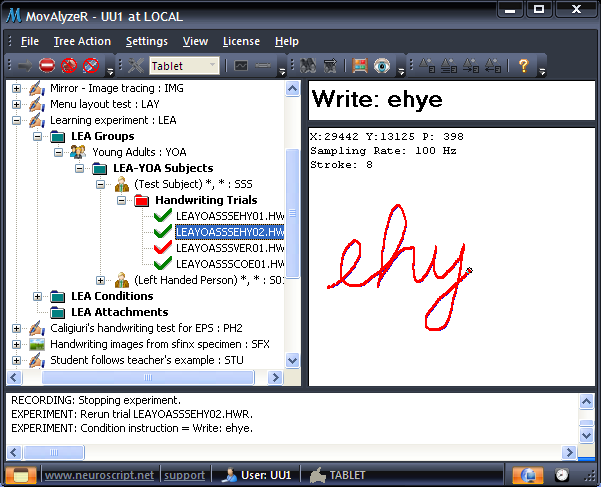
\includegraphics[width=0.7\textwidth]{figures/neuroscript.png}
    \caption{Программное средство <<ScriptAlyzeR>>}
    \label{fig:domain:analogs:neuro_script}
\end{figure}

\subsubsection{Graphology}
\label{sub:domain:analogs:graphology} 

Программное средство <<Graphology>> является приложением для операционной системы Android, разработанным компанией <<LH Apps>>~\cite{analogs_graphology}.

Программное средство <<Graphology>> предназначено для анализа почерка и определения характеристик личности. Алгоритм работы программы основан на обширных исследованиях и был создан при консультации профессиональных экспертов графологии. Пользовательский интерфейс приложения представлен на рисунке~\ref{fig:domain:analogs:graphology}.

Основными возможностями ПС являются:
\begin{itemize}
  \item поддержка ОС Android;
  \item многофакторная оценка параметров личности (почерк, подпись);
  \item выполнение анализа без доступа в интернет.
\end{itemize}

Основными недостатками ПС являются:
\begin{itemize}
  \item поддержка только ОС Android;
  \item поддержка только английского языка;
  \item для ввода образцов почерка используется экран смартфона, что приводит к искажению в написании символов при низком разрешении и без использование стилуса.
\end{itemize}

\begin{figure}[ht]
    \centering
    
\includegraphics[width=0.7\textwidth]{figures/graphology_analog.jpeg}
    \caption{Программное средство <<Graphology>>}
    \label{fig:domain:analogs:graphology}
\end{figure}

\subsubsection{Signature Analysis}
\label{sub:domain:analogs:signature_analysis} 

Программное средство <<Signature Analysis>> является приложением для операционной системы Android, разработанным компанией <<Beyond Consultancy Services>>~\cite{analogs_signature_analysis}.

Программное средство <<Signature Analysis>> предназначено для определения характеристик личности по образцу подписи. В разработке участвовал графолог с многолетним опытом, выступающей в качестве консультанта многих крупных компаний.  Пользовательский интерфейс приложения представлен на рисунке~\ref{fig:domain:analogs:signature_analysis}.

Основными возможностями ПС являются:
\begin{itemize}
  \item поддержка ОС Android;
  \item широкий спектр анализируемых параметров подписи (скорость, давление, длины, направления);
\end{itemize}

Основными недостатками ПС являются:
\begin{itemize}
  \item поддержка только ОС Android;
  \item платный анализ каждой подписи (0,83 \$);
  \item для работы необходимо интернет соединение;
  \item для ввода образцов почерка используется экран смартфона, что приводит к искажению в написании символов при низком разрешении и без использование стилуса.
\end{itemize}

\begin{figure}[ht]{}
    \centering
    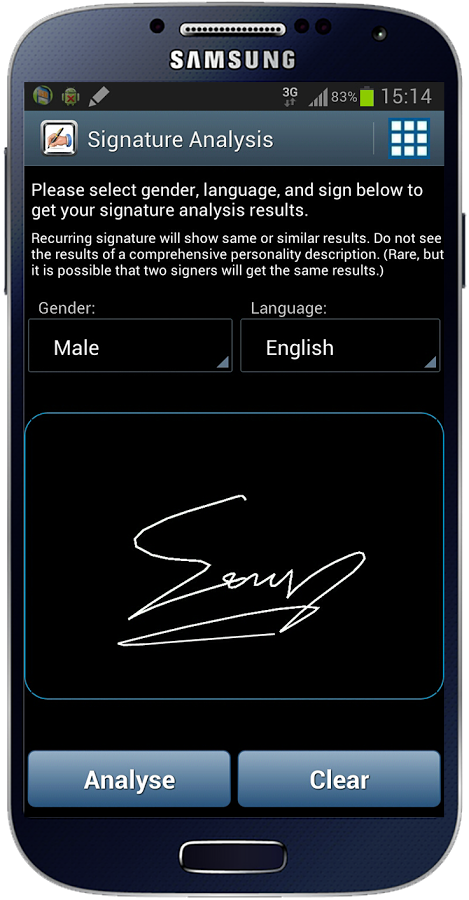
\includegraphics[height=0.4\textheight]{figures/analog_signature_analysis.png}
    \caption{Программное средство <<Signature Analysis>>}
    \label{fig:domain:analogs:signature_analysis}
\end{figure}

\subsubsection{My Graphology}
\label{sub:domain:analogs:my_graphology}

Программное средство <<My Graphology>> является приложением для операционной системы Android, разработанным компанией <<PENS>>~\cite{analogs_my_graphology}. Пользовательский интерфейс приложения представлен на рисунке~\ref{fig:domain:analogs:my_graphology}.

\begin{figure}[h]
    \centering
    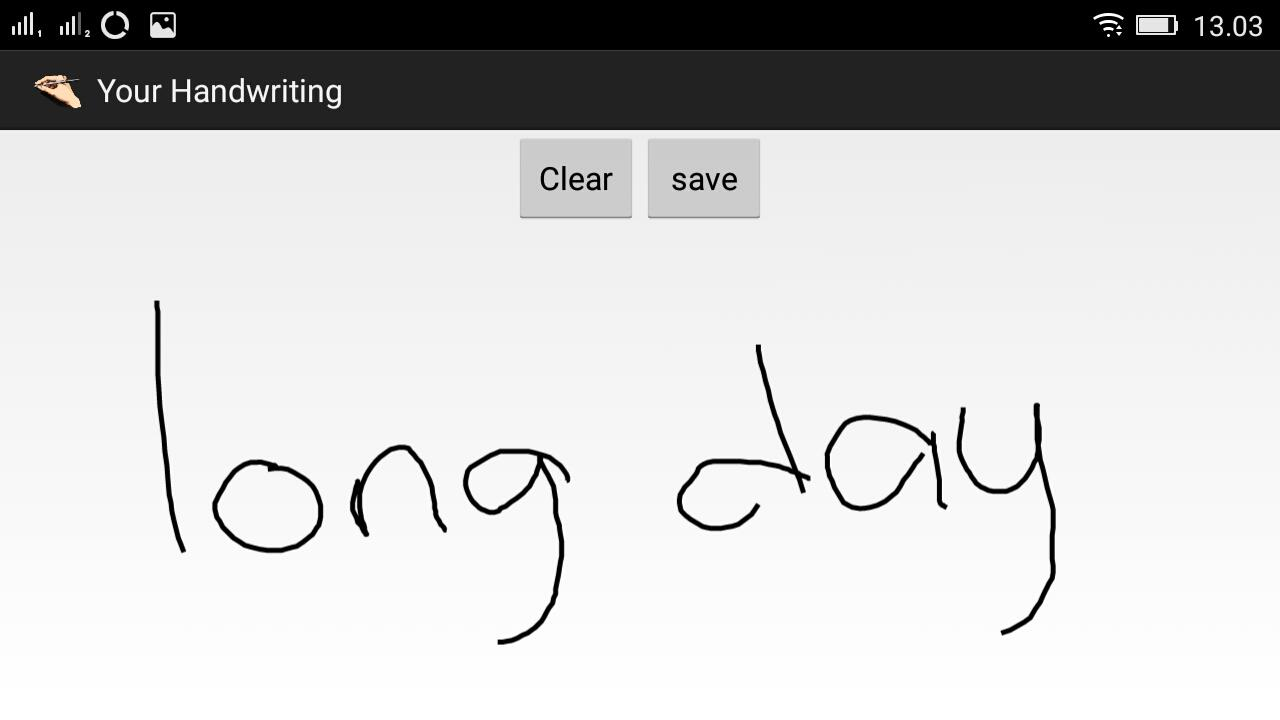
\includegraphics[width=0.4\textheight]{figures/analog_my_graphology.jpeg}
    \caption{Программное средство <<My Graphology>>}
    \label{fig:domain:analogs:my_graphology}
\end{figure}

Основными возможностями ПС являются:
\begin{itemize}
  \item поддержка ОС Android;
  \item использование для ввода экрана или фотографии почерка;
  \item выполнение анализа без доступа в интернет.
\end{itemize}

Основными недостатками ПС являются:
\begin{itemize}
  \item поддержка только ОС Android;
  \item в разработке не участвовали эксперты графологи;
  \item поддержка только испанского языка интерфейса.
\end{itemize}

\subsubsection{GRAPHOLOGY signature analysis}
\label{sub:domain:analogs:graphology_sign_analysis}

Программное средство <<GRAPHOLOGY signature analysis>> является приложением для операционной системы Android, разработанным компанией <<DokThor>>~\cite{analogs_graphology_sign_analysis}. Программное средство <<GRAPHOLOGY signature analysis>> предназначено для определения характеристик личности по образцу подписи. Пользовательский интерфейс приложения представлен на рисунке~\ref{fig:domain:analog:graphology_sign_analysis}.

\begin{figure}[h]
    \centering
    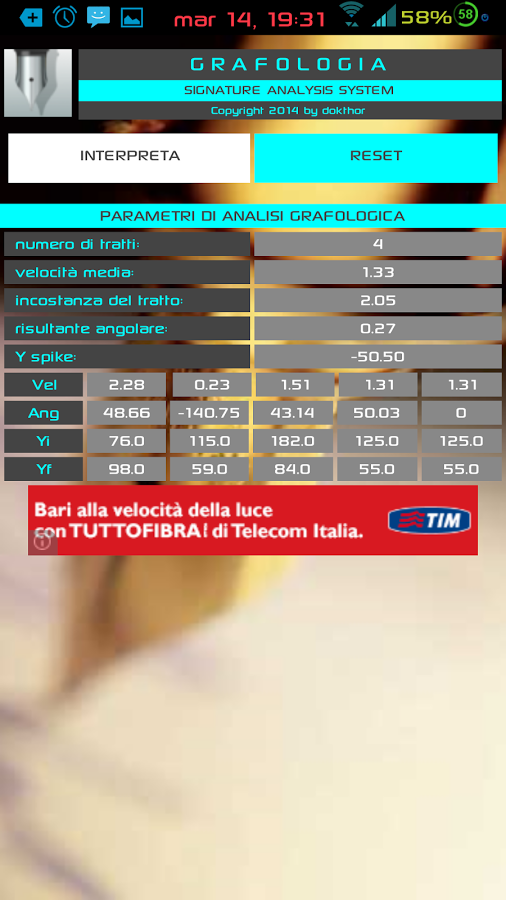
\includegraphics[height=0.5\textheight]{figures/analog_graphology_sign_analysis.png}
    \caption{<<GRAPHOLOGY signature analysis>>}
    \label{fig:domain:analog:graphology_sign_analysis}
\end{figure}

Основными возможностями ПС являются:
\begin{itemize}
  \item поддержка ОС Android;
  \item выполнение анализа без доступа в интернет;
  \item предоставление характеристик личности по 5 основным критериям.
\end{itemize}

Основными недостатками ПС являются:
\begin{itemize}
  \item поддержка только ОС Android;
  \item в разработке не участвовали эксперты графологи;
  \item механизм ввода подписи неочевиден;
  \item для ввода образцов почерка используется экран смартфона, что приводит к искажению в написании символов при низком разрешении и без использования стилуса.
\end{itemize}

\subsubsection{Graphology Lite}
\label{sub:domain:analogs:graphology_lite}

Программное средство <<Graphology Lite>> является приложением для операционной системы Android, разработанным компанией <<Hyperborea>>~\cite{analogs_graphology_lite}. Пользовательский интерфейс приложения представлен на рисунке~\ref{fig:domain:analogs:graphology_lite}.

\begin{figure}[h]
    \centering
    
\includegraphics[height=0.5\textheight]{figures/analog_graphology_lite.png}
    \caption{Программное средство <<Graphology Lite>>}
    \label{fig:domain:analogs:graphology_lite}
\end{figure}

Основными возможностями ПС являются:
\begin{itemize}
  \item поддержка ОС Android;
  \item выполнение анализа без доступа в интернет;
  \item использование для ввода экрана или фотографии почерка.
\end{itemize}

Основными недостатками ПС являются:
\begin{itemize}
  \item поддержка только ОС Android;
  \item в разработке не участвовали эксперты графологи;
  \item бесплатная версия позволяет произвести анализ только одного образца (платная версия стоит 1.05 \$).
\end{itemize}

В результате анализа было выявлено, что текущие аналоги, описанные в данном разделе, не обладают следующими возможностями, необходимыми для эффективного практического использования:
\begin{itemize}
  \item поддержка ОС Linux и MacOS;
  \item поддержка русского языка интерфейса;
  \item взимание платы за использование;
  \item поддержка механизма контроля доступа.
\end{itemize}

\subsection{Анализ литературных источников}
\label{sub:domain:literary_sources}

Публикации и научные статьи на темы схожие с темой данной работы можно условно разделить по следующим признакам:
\begin{itemize}
  \item метод сегментации изображения;
  \item метод классификации признаков изображения.
\end{itemize}

Метод сегментации изображения является неотъемлемой частью алгоритмов обработки рукописного текста, будь это распознавание или анализ. От качества сегментации напрямую зависит качество работы всего алгоритма поэтому выбор метода сегментации является важным этапом.

В рассмотренной литературе предлагаются следующие алгоритмы сегментации рукописного текста:
\begin{itemize}
  \item преобразования Хафа~\cite{louloudis_gatos_pratikakis_halatsis};
  \item нечеткие интервалы~\cite{louloudis_gatos_pratikakis_halatsis};
  \item нечеткий и адаптивный рекурсивный метод наименьших \mbox{квадратов~\cite{louloudis_gatos_pratikakis_halatsis};}
  \item статистические методы (средний интервал между строками)~\cite{gomathi_umadevi_mohanavel};
  \item метод Лоулодиса-Гатоса-Пратикакиса-Халатсиса (LGPH)~\cite{louloudis_gatos_pratikakis_halatsis};
  \item проецирование контуров~\cite{louloudis_gatos_pratikakis_halatsis}.
\end{itemize}

Преобразования Хафа являются мощным инструментом компьютерного зрения, позволяющим извлекать элементы из изображения. Данный метод позволяет достичь высокой точности сегментации текста, однако требует больших вычислительных затрат в связи с объемом вычислений и использованием тригонометрических функций при вычислении.

Метод рекурсивных нечетких и адаптивных наименьших квадратов, так же как и преобразования Хафа, широко используется для выделения областей изображения благодаря высокому качеству работы и устойчивости к шумам и искажениям, однако вычислительная стоимость данных методов относительно велика.

Метод Лоулодиса-Гатоса-Пратикакиса-Халатсиса показывает очень хорошие результаты сегментации и по результатам исследований превосходит по качеству и времени работы все приведенные выше алгоритмы, однако он пока находится в состоянии исследования и не имеет реальных примеров реализации и использования в практических проектах.

Методы проецирования контуров и нечетких интервалов хорошо подходят для распознавания печатного текста, но дают плохие результаты при распознавании рукописного из-за динамически изменяющихся интервалов между символами,строками и словами.

Статические методы основаны на разбиении изображении в зависимости от распределения средней яркости частей изображения, качества работы данных методов ниже чем у преобразований Хафа или рекурсивных методов на основе наименьших квадратов, но время работы намного меньше благодаря меньшему количеству вычислений и быстрым операциям сложению и делению.

В разрабатываемом программном средстве не требуется высокая точность распознавания, как например для распознавания текста, в то время как программное средство может работать с большим количеством изображений одновременно и быстродействие важно. Исходя из этого в качестве алгоритма сегментации будет использоваться статический метод.

Не менее важным является алгоритм классификации, так как именно он будет устанавливать соответствие между параметрами текста и психологическими характеристиками, например силой нажима и степенью наклона символа.

В рассмотренной литературе предлагаются следующие алгоритмы классификации признаков рукописного текста:
\begin{itemize}
  \item нейронные сети~\cite{champa_ananda_kumar_ann, grewal_prashar, gabrani_solomon_dviwe,puri_lakhwani, dang_kumar, kathait_singh};
  \item мешок особенностей~\cite{rothacker_bag_of_features};
  \item метод опорных векторов~\cite{slideshare_khandelwal_garg, gabrani_solomon_dviwe, prasad_singh_sapre};
  \item метод основанный на правилах~\cite{champa_ananda_kumar_rule_base}.
\end{itemize}

Метод основанный на правилах заключается в последовательной проверке соответствия параметров почерка набору правил <<если"=то>>. Как пример можно привести правило <<Если строки наклонены влево и сила нажима слабая, то человек пессимист не склонный к выражению эмоций>>. Данный подход основан только на описании графологических метод, обладает высокой скоростью и не требует обучения. Однако требуется определение границ значений анализируемых параметров, а так же количество правил экспоненциально растет с количеством параметров и их возможных значений, так для двух параметров с тремя значениями каждого понадобиться 9 правил~\cite{champa_ananda_kumar_rule_base}, а для пяти параметров уже 243.

Метод основанный на <<мешке особенностей>> состоит в составлении <<словаря слов>> на основе большой базы изображений. Данный словарь будет содержать фрагмент изображения описанный каким-либо дескриптором, например SIFT, и частоту появления этого фрагмента. По сути данный метод рассматривает задачу определения психологических параметров как задачу категоризации. Основными недостатками данного метода является необходимость в сборе и ручной обработке, определения параметров личности экспертами графологами, огромной базы изображений, т.к. все образцы почерка достаточно похожи и сложно выделить отличительные признаки.

Использование нейронных сетей является хорошим решением благодаря способности сети обобщать данные, а использование обратного распространения ошибок позволяет добиться очень хорошего качества распознавания. Однако выбор оптимальной структуры сети и функции активации нейронов является нетривиальной задачей, так же время обучения и распознавания относительно велико.

Метод опорных векторов основан на нахождении границы классов максимально удаленной от их экземпляров. К его достоинствам относиться хорошее качество распознавания, высокая скорость обучения и классификации. Однако необходим большой объем обучающей выборки, такой чтобы каждый из возможных наборов признаков встречался хотя бы раз. Так же вопрос выбора оптимального типа ядер схож с выбором функции активации для нейронных сетей.

Основываясь на проведенном анализе и объеме обучающей выборки, ($\sim$ 1500 образцов), было принято решение использовать метод опорных векторов в качестве классификатора. Точность классификации нейронных сетей и метода опорных векторов примерно равны, однако скорость обучения и распознавания у опорных векторов выше, что так же повлияло на решение.

\subsection{Обоснование выбора языка и сред разработки}
\label{sec:techs:intro}

Выбор технологий является важным предварительным этапом разработки сложных информационных систем. Платформа и язык программирования, на котором будет реализована система, заслуживает большого внимания, так как множество исследований показали, что выбор языка программирования значительно влияет на производительность труда программистов и качество создаваемого ими кода~\cite[c.~59]{mcconnell_2005}.

На выбор технологий повлияли следующие факторы:
\begin{itemize}
\item программное средство должно быть выполнено в виде клиент"=серверного приложения;
\item разрабатываемое ПО должно работать на операционных системах Linux, MacOS и Windows;
\item разработчик имеет опыт работы с объектно"=ориентированными и функциональными языками программирования.
\end{itemize}

\subsubsection{Язык программирования Scala}
\label{sub:techs:scala}
Scala – мультипарадигмальный, компилируемый, строго типизированный язык программирования, спроектированный кратким и безопасным для простого и быстрого создания компонентного программного обеспечения, сочетающий возможности функционального и объектно-ориентированного программирования~\cite{wiki_scala}.

Scala поддерживает объектно-ориентированную и функциональную парадигмы программирования, но доминирующей является объектно-ориентированная. Язык был выпущен для общего пользования на платформе JVM и .NET, так же создан LLVM-компилятор (Scala Native) и транслятор в JavaScript (ScalaJS).

Отличительные особенности языка Scala:
\begin{itemize}
  \item Лаконичность. Код на Scala в средней вдвое короче кода на Java.
  \item Открытый исходный код. Код стандартной библиотеки опубликован к открытом доступе на портале GitHub и любой желающий, при наличии желания и способностей, может стать участником проекта.
  \item Высокий уровень абстракции. В стандартной библиотеке реализованы большинство типичных операции над строками и коллекциями, в частности итерация по элементам коллекции инкапсулирована в методах map, filter, flatMap. Так же выражение for трансформируется в вызов выше описанных методов, что позволяет использовать в нем пользовательские контейнеры и типы данных. 
  \item Платформонезависимость. Код языка компилируется в JVM байт-код и может исполняться на любой платформе поддерживающей JVM.
  \item Строгая система типов. Позволяет выявить многое ошибки еще на стадии компиляции.
  \item Объектно-ориентированность. Язык поддерживает основные концепции объектно-ориентированного программирование (наследование, инкапсуляция, полиморфизм).
  \item Функциональность. Язык поддерживает основные концепции функционального программирование (функции высших порядков, сопоставление с образцов, <<ленивые>> вычисления).
  \item Расширяемость. В языке присутствуют механизм (неявные преобразования) позволяющий расширять функционал стандартных классов и сторонних библиотек.
  \item Использование Java-кода. Возможно использовать не только библиотеки написанные на Java, но и классы написанные на Java в Scala-проекте, но отсутствует полная обратная совместимость.
  \item Широкий набор библиотеки. Стандартная библиотека Scala содержит классы для работы с вводом-выводом, регулярными выражениями, параллельной обработки, работы со строками, коллекции. Так же существует большое количество сторонних библиотек.
\end{itemize}

\paragraph{Объектно-ориентированное программирование}
Объектно-ориентированная парадигма программирования играет в языке важную роль. Стандартная библиотека языка реализована в виде набора классов и примесей, а так же модульность обеспечивается классами и пакетами~\cite{horsman_scala}.

Особенности Scala с точки зрения объектно"=ориентированной \mbox{парадигмы:}
\begin{itemize}
  \item статическая сильная полная типизация с автоматическим \mbox{выведением типов;}
  \item наследование, в том числе использование примесей (Traits);
  \item полиморфизм;
  \item инкапсуляция;
  \item конструкторы, деструкторы;
  \item все математические операторы являются методами;
  \item гибкое управление доступом к полям и методам;
  \item метапрограммирование;
  \item объекты компаньоны (используются для инкапсуляции статических полей и методов).
\end{itemize}

\paragraph{Функциональное программирование}
Особенности Scala с точки зрения функциональной парадигмы:
\begin{itemize}
  \item функции высших порядков;
  \item функции объект первого класса;
  \item оптимизация хвостовой рекурсии;
  \item сопоставление с образцов;
  \item поддержка неизменяемых структур данных;
  \item функциональные комбинаторы и композиции;
  \item частичное применение функции;
  \item <<ленивые>> вычисления;
  \item структурное переиспользование неизменяемых коллекций.
\end{itemize}

Основываясь на выше перечисленных факторах было принято решение использовать в качестве основного языка программирования Scala как современный, активно набирающий популярность язык, поддерживающий функциональную и объектно"=ориентированную парадигмы программирования. Так же благодаря интеграции с Java, части кода требующего быстродействия могут быть реализованы на этом языке.

\subsubsection{Фреймворк Akka}
\label{sec:techs:akka}

Akka – набор прикладных библиотек (фреймворк) предоставляющий высокоуровневый интерфейс для разработки, развертывания и отладки систем акторов.

Основными достоинствами фреймворка Akka являются:
\begin{itemize}
  \item Простота интерфейса, высокая степень абстракции.
  \item Устойчивость к отказам, благодаря механизму супервизор.
  \item Масштабируемость. Простата добавления акторов в систему и развертывания компонентов на другой машине.
  \item Высокая скорость работы и степень параллелизма, благодаря использованию модели акторов;
  \item Минимально количество блокирующих операций, отсутствие общего изменяемого состояния.
\end{itemize}

\begin{figure}[ht]
    \centering
    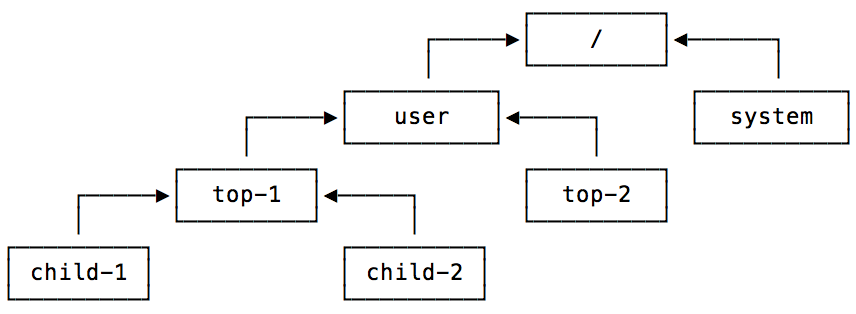
\includegraphics[width=0.7\textwidth]{figures/actors_hier.png}
    \caption{Иерархия акторов}
    \label{fig:techs:akka:actor_hierar}
\end{figure}

\paragraph{Модель акторов}
\label{sec:techs:akka:actor_model}
Модель акторов - модель параллельных вычислений, основанная на взаимодействии изолированных примитивов, взаимодействующих по средствам получения и отправки сообщений. Впервые была предложена в 1973 году~\cite{hewitt_bishop_steiger_actor_model}.

Основным понятием данной модели является «актор». Согласно модели актор лишен состояния и информации о структуре системы (количество братьев и родителей).

На рисунке~\ref{fig:techs:akka:actor_hierar} представлена иерархия акторов, в данном случае <<top-1>> является родителем для акторов <<child-1>> и <<child-2>>. Актор <<top-1>> выполняет функции супервизора и в случае ошибки в дочерних акторах получает соответствущее сообщение и может принимать решение для его исправлению, например перезапустить актор. Так же в случае необходимости можно делегировать принятие решения родительскому актору, в данном примере <<user>>. 
\begin{figure}[ht]
    \centering
    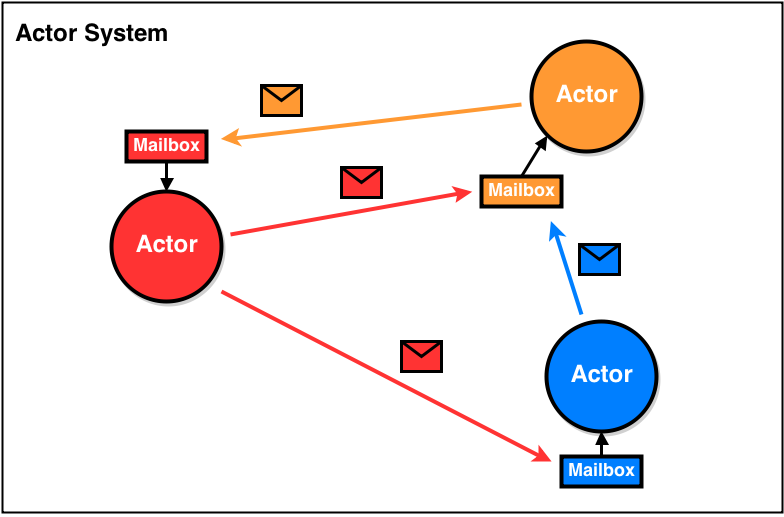
\includegraphics[width=0.7\textwidth]{figures/actor_model.png}
    \caption{Пример взаимодействия акторов}
    \label{fig:techs:akka:actor_model:comulication}
\end{figure}

Как видно на рисунке~\ref{fig:techs:akka:actor_model:comulication}, отсутствует прямое взаимодействия акторов между собой, вся коммуникация осуществляется при помощи передачи сообщений. В совокупности с использованием неизменяемых структур данных, механизм сообщений делает всю работу системы акторов априорно асинхронной и неблокирующей.

При получении сообщения актор может:
\begin{itemize}
  \item отправить конечное число сообщений другим акторам;
  \item создать конечное число новых акторов;
  \item выбрать поведение, которое будет использоваться при обработке следующего полученного сообщения.
\end{itemize}

Данный подход позволяет теоретически полностью избежать блокировок благодаря отсутствию прямых вызовов методов актора и даже механизма ожидания ответа, позволяет добиться прироста производительности сопоставимого с количеством ядер процессоров в среде исполнения, чего невозможно добиться при использовании классической модели параллельности на основе потоков и блокировках при доступе к общему изменяемому состоянию.

Перечисленные достоинства, в особенности устойчивой к отказам и простота масштабирования, являются крайне важными при реализации архитектуры на основе микросервисов. Исходя из выше перечисленного, для обеспечения параллельной обработки данных будет использоваться набор прикладных библиотек (фреймворк) Akka. 

\subsubsection{Фреймворк Spray}
\label{sec:techs:spray}

Spray – набор прикладных библиотек (фреймворк), предназначенный для реализации веб-приложений, написанный на Scala. Фреймворк базируется на описанном выше фреймворке Akka и реализует асинхронное распределение запросов пользователя на иерархию акторов. 

Основными достоинствами фреймворка Spray являются:
\begin{itemize}
  \item полная асинхронность, отсутствие блокировок (весь интерфейс полностью асинхронный);
  \item высокая производительность (используются специальные низкоуровневые компоненты);
  \item модульность (весь интерфейс полностью асинхронный);
  \item легковесность (включаются только необходимые модули).
\end{itemize}

Данный набор библиотек достаточно молодой и еще не получил широкого распространения в коммерческой разработке, что может сказаться на стабильности работы и производительности, однако разработчики быстро устраняют дефекты и выпускают новые версии фреймворка раз в месяц. Использование данного фреймворка позволит упростить и ускорить разработку, отладку и последующее сопровождения благодаря использования одной концепции с предыдущим фреймворком.
Альтернативой является использование таких фреймворком как Lift и Play, однако они не имеют встроенной поддержки модели акторов, а так же требует дополнительных компонентов, контейнера Сервлетов, например Tomcat или Jetty, для развертывания.

Исходя из выше перечисленного, для реализации серверной части приложения будет использоваться набор прикладных библиотек Spray, так как несмотря на возможные недоработки он хорошо встраивается в экосистему данного проекта.
\subsection{Постановка задачи}
\label{sec:domain:requirements}

В результате выполнения дипломного проекта должно быть разработано программное средство определения психологических параметров личности по образцу почерка, реализующее процедуры выделения признаков почерка из изображения и их классификацию, а так же механизм авторизации для обеспечения секретности данных.

Разрабатываемое программное средство должно выполнять следующие функции:
\begin{itemize}
  \item регистрация пользователя;
  \item авторизация пользователя;
  \item просмотр сохраненных образцов почерка;
  \item удаление сохраненных образцов почерка;
  \item добавление нового образца почерка;
  \item выделение признаков образца почерка;
  \item определение параметров личности;
  \item обновление образцов почерка.
\end{itemize}

К разрабатываемому программному средству предъявляются следующие требования:
\begin{itemize}
  \item разрабатываемое ПО должно работать на операционных системах Linux, MacOS и Windows;
  \item модуль программного срества требует 512 MB оперативной памяти;
  \item программное средство должно быть выполнено в виде клиент"=серверного приложения;
  \item программное средство должно поддерживать русский язык \mbox{интерфейса;}
  \item выходными данными являются документы в формате JSON;
  \item входными данными являются изображения в форматах jpeg, bmp и png.
\end{itemize}   

% Глава 2 Функциональные требования
\section{Функциональные требования}
\label{sec:freq}

Основываясь на требованиях изложенных в разделе \ref{sec:domain:requirements} и диаграмме вариантов использования разработана спецификация требований к разрабатываемому ПС.

\begin{figure}[ht]
\centering
    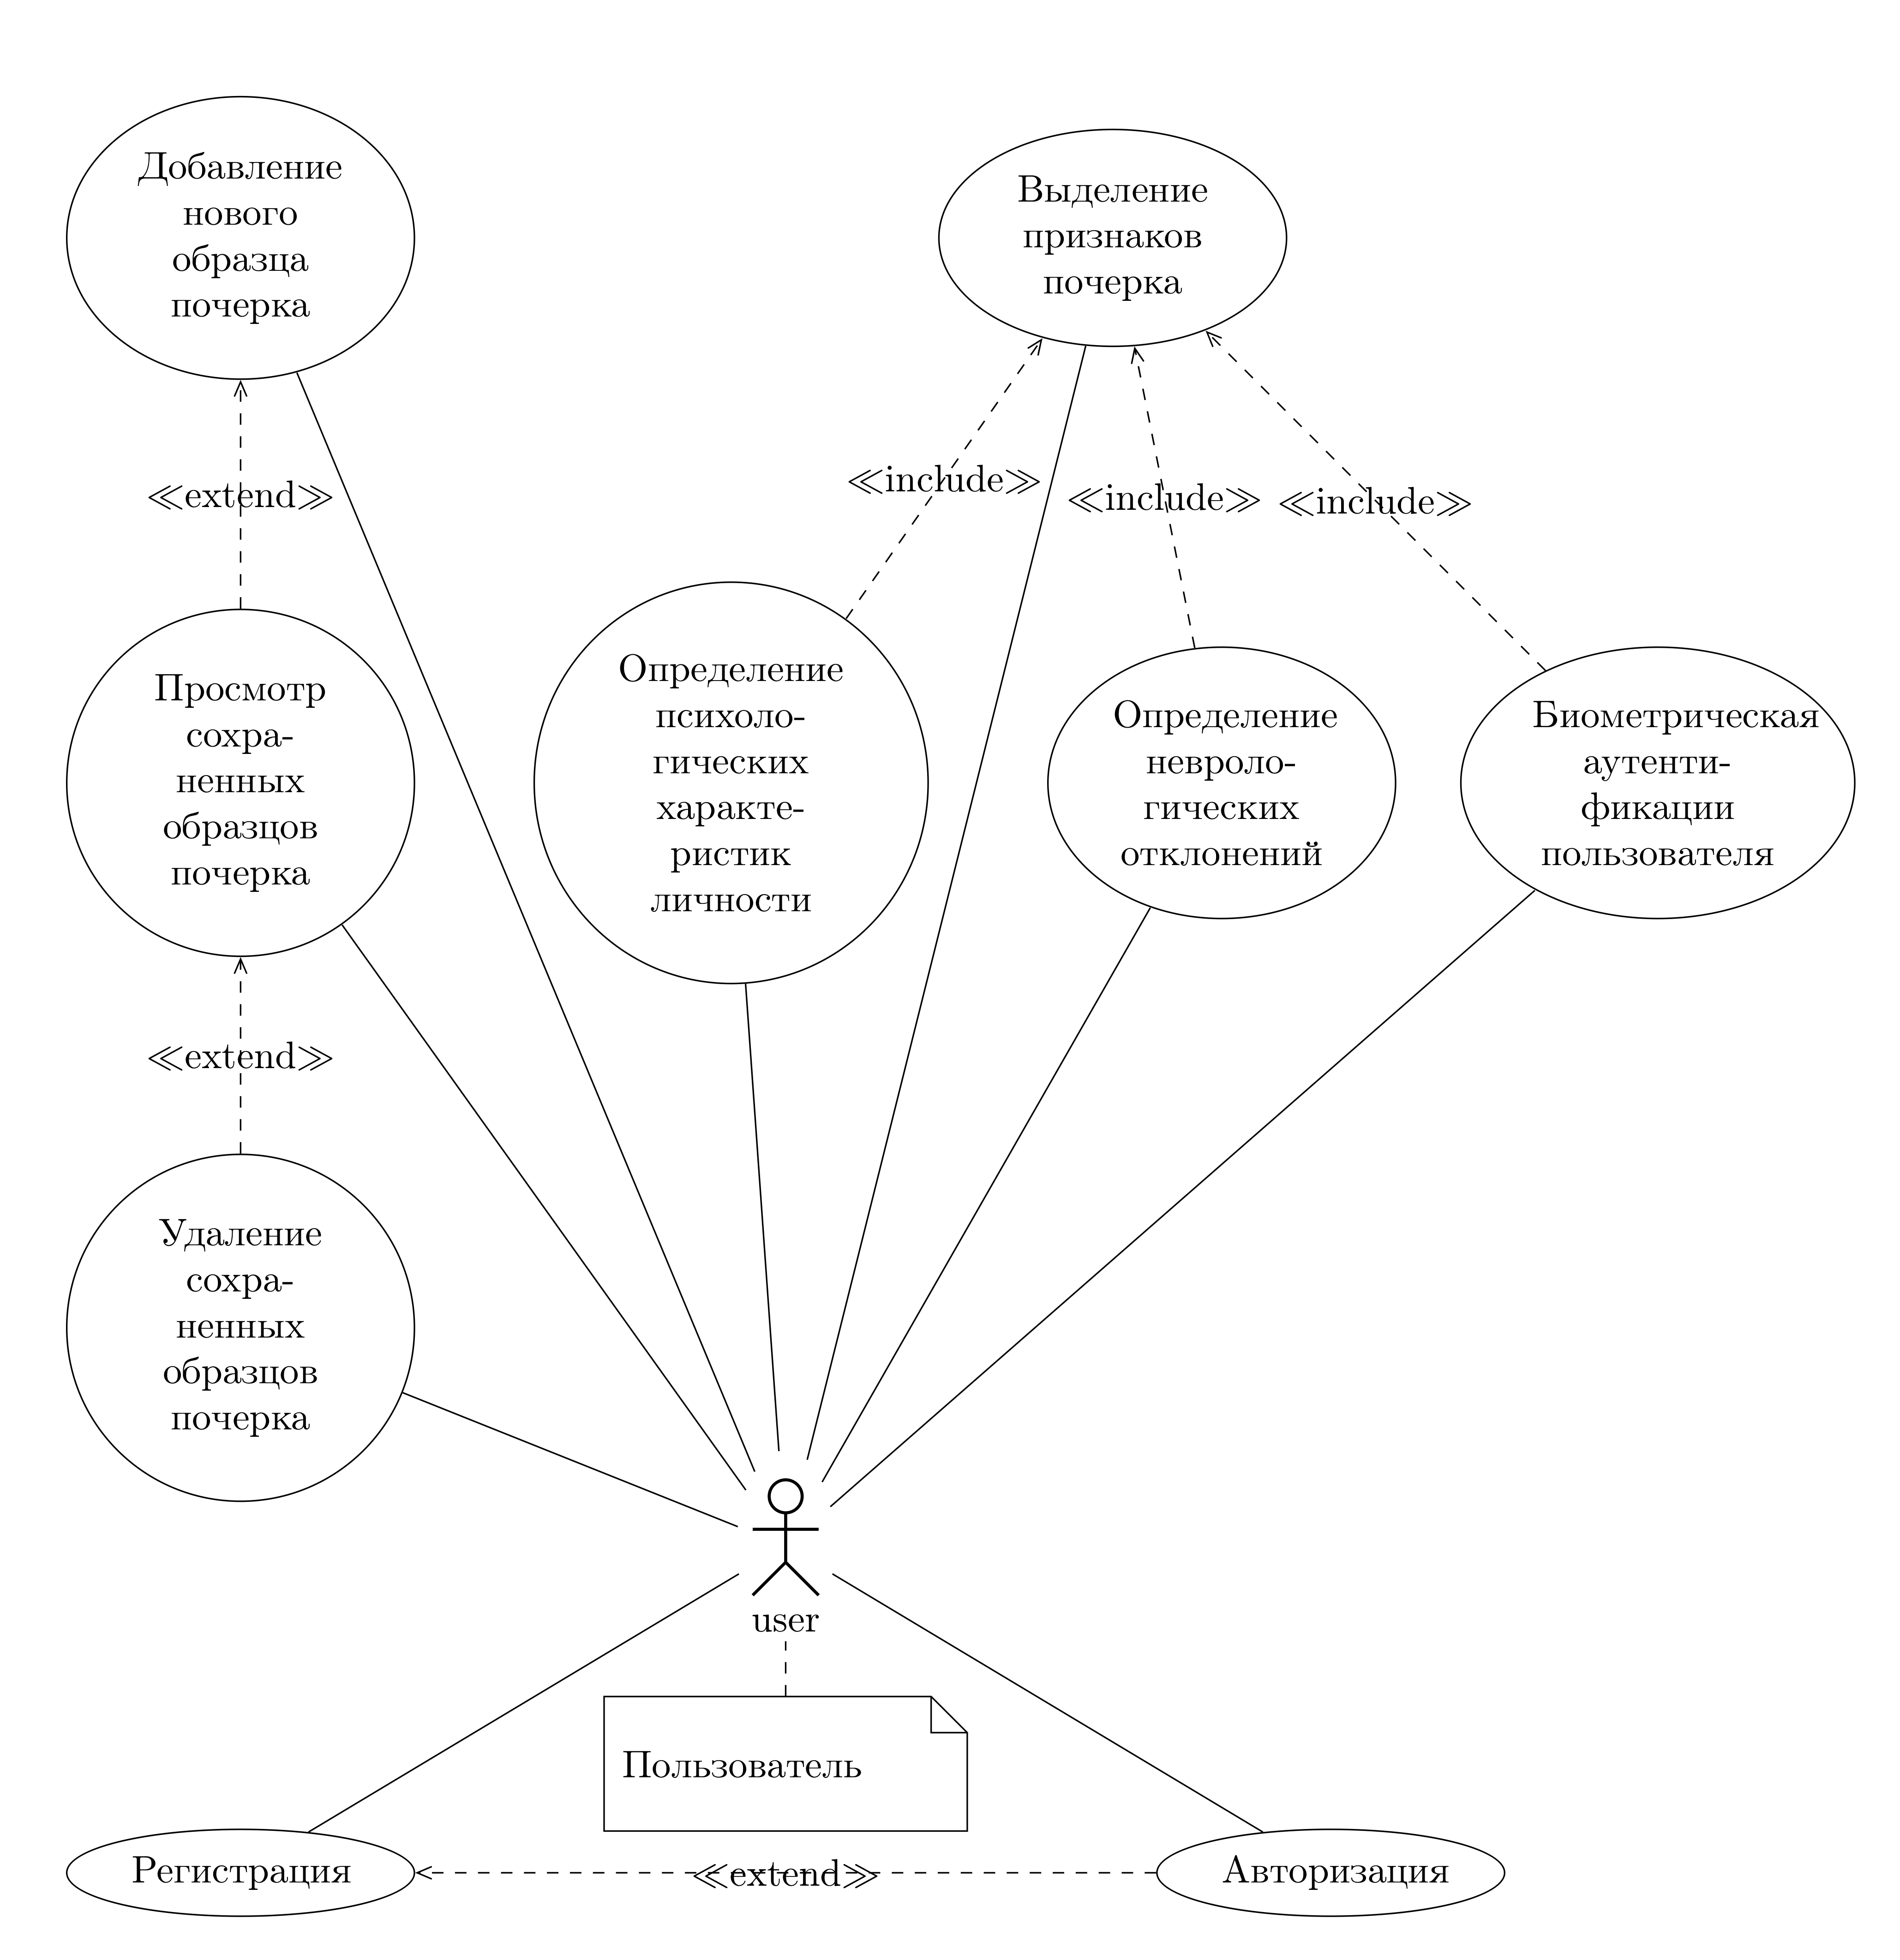
\includegraphics[scale=0.53]{figures/use_case.png}  
    \caption{Диаграмма вариантов использования}
  \label{fig:freg:usecase}
\end{figure}

\subsection{Регистрация пользователя}
\label{sec:freq:reg}
\begin{itemize}
	\item возможность регистрации должна быть доступна из пользовательского веб-интерфейса;
	\item пароль при регистрации должен проверяться на сложность(должен содержать не менее 8 символов в верхнем и нижнем регистрах и цифры);
	\item авторизационные данные пользователя должны передаваться по защищенному соединению;
\end{itemize}

\subsection{Авторизация пользователя}
\label{sec:freq:auth}
\begin{itemize}
	\item авторизационные данные пользователя должны передаваться по защищенному соединению;
	\item пароль пользователя не должен передаваться в явном виде (вычисления хеша в браузере);
 	\item сообщение об ошибке при вводе неверное логина или пароля не должно сообщать что именно введено неправильно.
\end{itemize}

\subsection{Просмотр сохраненных образцов почерка}
\label{sec:freq:show}
\begin{itemize}
	\item список ранее загруженных образцов доступен на главной странице пользователя;
	\item изображение и дополнительная информация(признаки почерка, параметры личности) должны загружаться только после выбора изображения из списка;
	\item пользователь имеет возможность запустить процесс выделения признаков почерка;
	\item пользователь имеет возможность запустить процесс параметров личности, если процесс выделения признаков почерка еще не был выполнен, и по окончанию начнется процесс определения параметров личности;
\end{itemize}

\subsection{Удаление сохраненных образцов почерка}
\label{sec:freq:delete}
\begin{itemize}
	\item возможность удаления сохраненных образцов почерка должна быть доступна из пользовательского веб-интерфейса страница просмотра образца;
	\item при удалении должно запрашиваться подтверждение действия пользователя с сообщением о последствиях;
	\item реальное удаление образца происходит через неделю после подтверждения удаления пользователем (возможность восстановить файл при ошибочном удалении).
\end{itemize}

\subsection{Добавление нового образца почерка}
\label{sec:freq:add}
\begin{itemize}
	\item возможность добавить новый образец доступна на главной странице пользователя;
	\item возможно добавить образцы в форматах jpg(jpeg), bmp и png;
	\item добавляемый образце должен иметь размер более 0 и менее 10 MB;
	\item после добавления нового образца пользователь переходит на страницу просмотра образца;
\end{itemize}

\subsection{Выделение признаков образца почерка}
\label{sec:freq:extract_features}
\begin{itemize}
	\item возможность выделение признаков образца почерка должна быть доступна из пользовательского веб-интерфейса страница просмотра образца;
	\item до завершения выделения признаков на странице отображается индикатор отработки в виде вращающегося круга.
\end{itemize}

\subsection{Определение параметров личности}
\label{sec:freq:psiho_analysis}
\begin{itemize}
	\item возможность определение параметров личности должна быть доступна из пользовательского веб-интерфейса страница просмотра образца;
	\item до завершения определение параметров личности на странице отображается индикатор отработки в виде вращающегося круга.
\end{itemize}

\subsection{Пакетное добавление образцов почерка}
\label{sec:freq:package_add}
\begin{itemize}
	\item возможность пакетного добавить новый образцов доступна на главной странице администратора;
	\item процессы выделения признаков и параметров личности начинаются автоматически;
	\item до завершения обработки изображений на странице отображается индикатор отработки в виде вращающегося круга.
\end{itemize}

\subsection{Пользовательский интерфейс программного средства}
\begin{itemize}
	\item пользовательский интерфейс представляет собой Web-страницу;
	\item пользовательский интерфейс поддерживает русский и английский языки;
	\item возможность смены языка доступна пользователю на любой странице;
	\item поддержка Google Chrome и Firefox последних версий;
\end{itemize}

Поддержка операционных систем Windows, Linux, MacOS обеспечивается использование <<тонкого клиента>> и ограничена только поддержкой данными системами версий браузеров.
Разрабатываемое программное средство будет бесплатным для использования без ограничений на количество обрабатываемых и хранимых файлов.

% Глава 3 Проектирование архитектуры программного средства
\section{Проектирование программного средства}

Исходя из требований и современных стандартов разработки, программное средство должно обладать следующими свойствами:
\begin{itemize}
    \item модульность;
    \item простота горизонтального масштабирования;
    \item параллельная обработка данных;
    \item безопасность хранения конфиденциальных и личных данных.
\end{itemize}

Для соответствия выше описанным свойствам было принято решение разрабатывать программное средство в виде изолированных модулей и использовать архитектуру микросервисов. Так как использование монолитной архитектуры затруднит горизонтальное масштабирование и увеличит связность модулей, что усложнит последующее сопровождение. 

Разработанное программное средство состоит из следующих модулей, рисунок~\ref{fig:architecture:deployment}:
\begin{itemize}
    \item модуль выделения признаков почерка;
    \item модуль определения параметров личности;
    \item модуль контроля доступа;
    \item модуль управление образцами почерка;
    \item модуль доступа к базе данных.
\end{itemize}

Вышеописанные модули опираются на следующие группы классов, разработанные в рамках дипломного проекта:
\begin{itemize}
    \item Набор классов для сегментации изображения на строки, слова, символы и выделения признаков. Написан на языке Scala с использование сторонней библиотеки Tesseract.
    \item Набор классов машинного обучения (для классификации признаков текста). Написан на языке программирования Scala и содержит реализацию алгоритма основанного на методе опорных векторов (Support Vector Machine), подробнее рассмотрен в главе~\ref{sec:architecture:personal_parameters}.
    \item Набор классов для контроля доступа. Написана на языке Scala. Содержит классы для регистрации, авторизации и управлением сессией пользователя. Основан на стандарте JSON Web Token (JWT).
    \item Набор классов для организации доступа и хранения авторизационных данным пользователя и коллекции обработанных изображений.
\end{itemize}

Далее приведено подробное описание структуры и назначения каждого модуля.

\afterpage{
  \begin{landscape}
  \thispagestyle{lscape}
  \begin{figure}[t!]
  \centering
    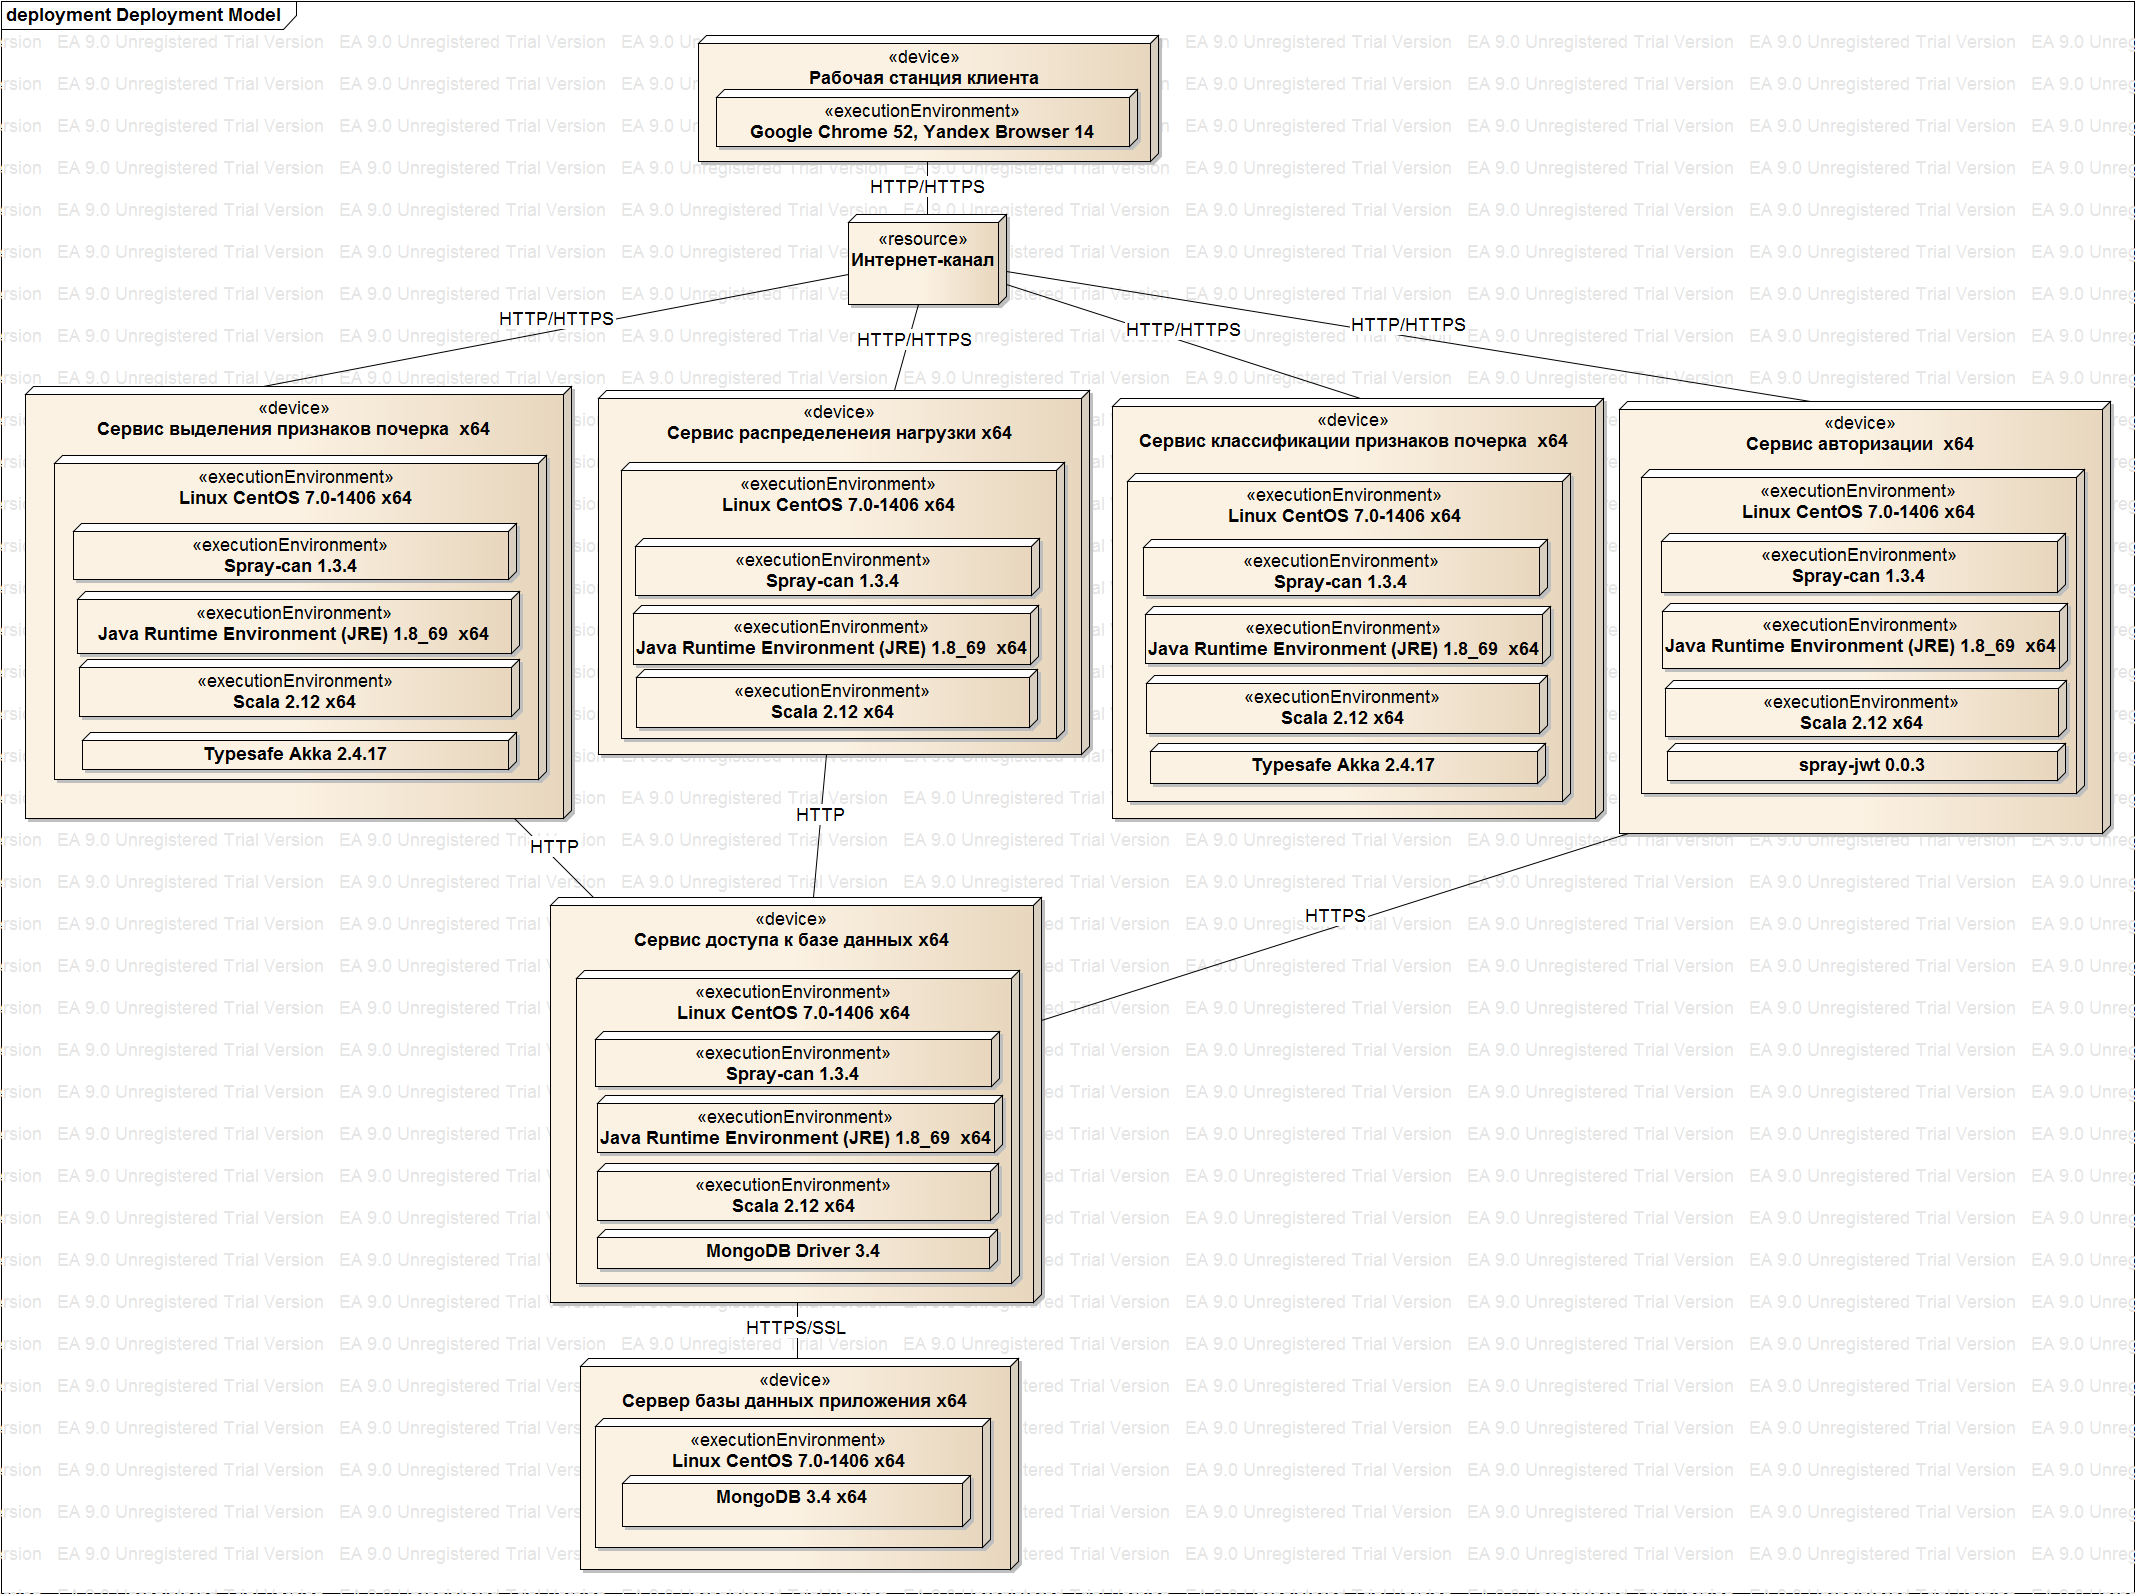
\includegraphics[scale=0.52]{figures/deployment_model.png}
    \caption{Диаграмма развертывания программного средства}
    \label{fig:architecture:deployment}
  \end{figure}
  \end{landscape}
}

\subsection{Модуль определения параметров личности}
\label{sec:architecture:personal_parameters}
Основываясь на анализе литературных источников в разделе~\ref{sub:domain:literary_sources} и спецификации требований, раздел~\ref{sec:freq:psiho_analysis}, было принято решение для определения параметров личности по признаком рукописного текста использовать классификатор на основе метода опорных векторов, широко используемого метода машинного обучения~\cite{manning_ir}, который при своей относительной простоте реализации, позволяет добиться очень неплохих результатов классификации.

Метод опорных векторов (\emph{SVM, support vector machine}) – семейство схожих алгоритмов обучения с учителем, использующихся для задач классификации и регрессионного анализа. Особым свойством метода опорных векторов является непрерывное уменьшение эмпирической ошибки классификации и увеличение зазора, поэтому метод также известен как метод классификатора с максимальным зазором~\cite{mitchell_ml, wiki_SVM}.

Параметры текста представляют собой непрерывные величины подчиняющиеся нормальному распределению, рисунок~\ref{fig:architecture:normal_pd}. Исходя их этого свойства использование полиномиальных однородных и неоднородных ядер не позволит достичь хороший результатов классификации, для достижения хороших результатов распознавания следует использовать в качестве ядер радиально-базисная функцию Гаусса~\cite{gauss_wiki}, формула~(\ref{eq:architecture:gaussian_core}). 

\begin{equation}
  \label{eq:architecture:gaussian_core}
  k(x, x^{'}) = \exp(-\frac{\left|\left| x - x^{'} \right|\right|}{2\sigma_{}^2})
\end{equation}
\begin{explanation}
где & $x^{'}$ & среднее значение параметра, рассчитанное для объектов, принадлежащих
классу $C$; \\
    & $ \sigma_{}^2 $ & дисперсия значения параметра объектов из класс $C$.
\end{explanation}

Дисперсия значения параметра представлена формулой~(\ref{eq:architecture:dispersion}).
\begin{equation}
  \label{eq:architecture:dispersion}
  \sigma_{}^2 = \frac{1}{n - 1} \sum\limits_{x \in C} (x_i - \overline{x_{}}^2)
\end{equation}

\begin{figure}[!h]
    \centering
    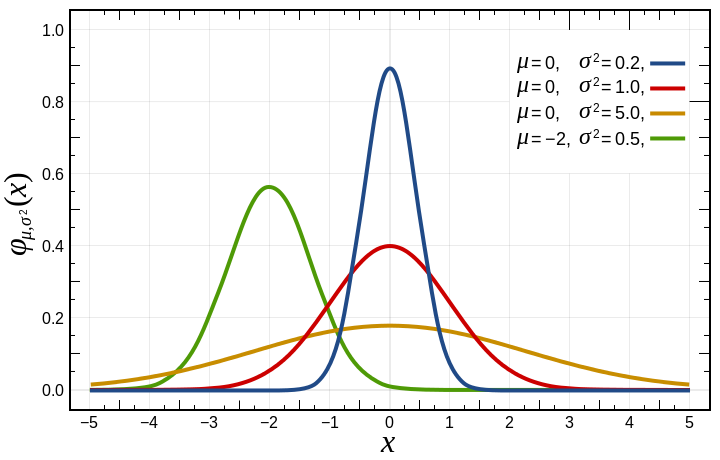
\includegraphics[width=0.85\textwidth]{figures/gauss.png}
    \caption{График функции плотности вероятности для нормального распределения}
    \label{fig:architecture:normal_pd}
\end{figure}

\subsection{Модуль выделения признаков почерка}
На основании требование сформированных в разделе~\ref{sec:freq:extract_features} основным функциями данного модуля является:
\begin{itemize}
  \item подготовка изображения к обработке (бинаризация, удаление \mbox{шумов);}
  \item сегментация текста (строки, слова, символы);
  \item выделения признаков почерка.
\end{itemize}

На это этапе обработки используется алгоритм линейной бинаризации по пороговому значению доминантного цвета, поскольку обработке подвергается образцы почерка с высокой вероятностью это будет цвет чернил.
Математическое выражение линейной бинаризации описывается формулой~(\ref{eq:architecture:liner_binarisation}).

\begin{equation}
  \label{eq:architecture:liner_binarisation}
 \left \{
  \begin{tabular}{l}
   x <  T, x = 0 \\
   x $ \geq $ T, x = 255
  \end{tabular}
   \right .
\end{equation}
\begin{explanation}
где & $ x $ & значения яркости цвета пикселя; \\
    & Т & порог бинаризации.
\end{explanation}

Для удаления шумов используется фильтр максимума - минимума. Алгоритм работы данного фильтра основан на замене текущего пикселя на пиксель с максимальной яркостью из его окрестности при первом проходе и на пиксель с минимальной при повторном. Данный алгоритм хорошо справляется с импульсными шумами и шумами типа <<соль и перец>>.

Следующий этапам является сегментация изображения, а первой стадией сегментации является сегментация строк. 
Задача выделения строк сводиться к нахождению верхних и нижних граней строк текста на исходном изображении. Алгоритм сегментации строк основывается на том, что средняя яркость в изображениях межстрочных промежутках существенно ниже средней яркости в изображениях текстовых строк~\cite{cv_text_image_segmentator}.

Первым этапом необходимо для всех строк пикселей исходного изображения находим их средние значения яркости, формула~(\ref{eq:architecture:line_medium_brigth}).
\begin{equation}
  \label{eq:architecture:line_medium_brigth}
  s_j = s_j(B) = \frac{1}{n}\cdot\sum\limits_{i=1}^{n} b_{ij}
\end{equation}

Затем необходимо определить среднюю яркость изображения, \mbox{формула~(\ref{eq:architecture:medium_brigth}).}
\begin{equation}
  \label{eq:architecture:medium_brigth}
  s(B) = \frac{1}{m}\cdot\sum\limits_{j=1}^{m} s_j(B)
\end{equation}

Средняя яркость в межстрочных интервалах невелика (после бинаризации близка к нулю). Поэтому яркость верхней границы можно выразить из яркости изображения, формула~(\ref{eq:architecture:line_up_interval_medium_brigth}).
\begin{equation}
  \label{eq:architecture:line_up_interval_medium_brigth}
  s^{t} = k_{t} \cdot s(B)
\end{equation}
\begin{explanation}
где & $ k_{t} $ & коэффициент от 0 до 1
\end{explanation}

Аналогично яркость нижней границы может быть выражена через яркость всего изображения, формула~(\ref{eq:architecture:line_down_interval_medium_brigth}).
\begin{equation}
  \label{eq:architecture:line_down_interval_medium_brigth}
  s^{b} = k_{b} \cdot s(B)
\end{equation}
\begin{explanation}
где & $ k_{b} $ & коэффициент от 0 до 1
\end{explanation}

Работа алгоритма заключается в последовательном просмотре массива средних значений $ (s_1,...,s_m) $ и выявлении множества пар индексов $ (s^t_i,s^b_i) $ строк пикселей соответствующих ниже приведенным условиям и следовательно являющимися верхней $ s^t_i $ и нижней $ s^b_i $ границам строк. 

Условия верхней границы текстовой строки:
\begin{itemize}
  \item яркость текущей строки пикселей превышает границу $ s^{t} $;
  \item яркость двух предыдущих строк пикселей ниже этой границы;
  \item яркость трех последующих строк выше границы $ s^{b} $.
\end{itemize}

Следовательно должно выполняться логическое условие описанное формулой~(\ref{eq:architecture:logic_up_interval}).
\begin{equation}
  \label{eq:architecture:logic_up_interval}
  (s_{i-2} < s^{t}) \wedge (s_{i-1} < s^{t}) \wedge (s_i > s^{b}) \wedge (s_{i+1} > s^{b}) \wedge (s_{i+2} > s^{b}) \wedge (s_{i+3} > s^{b})
\end{equation}

Условия нижней границы текстовой строки:
\begin{itemize}     
  \item было зафиксировано начало области;
  \item яркость текущей строки пикселей превышает границу $ s^{t} $;
  \item яркость последующей строки пикселей ниже границы $ s^{b} $.
\end{itemize}
     
Или:

\begin{itemize}
   \item было зафиксировано начало области;
   \item яркость трех последующих строк ниже границы $ s^{b} $.
\end{itemize}

Следовательно должно выполняться логическое условие описанное формулой~(\ref{eq:architecture:logic_down_interval}).
\begin{equation}
  \label{eq:architecture:logic_down_interval}
  ((s_{i+1} < s^{b}) \wedge (s_{i+2} < s^{b}) \wedge (s_{i+3} < s^{b}) \vee ((s_i > s^{t}) \wedge (s_{i+1} < s^{b})))
\end{equation}

Результатом работы алгоритма является множество пар индексов верхних и нижних границ строк. На основе этих данных можно рассчитать высоты строки (разность между индексами). Недостатком данного алгоритма является <<срезание>> символов, которые имеют высоту выше средней.

Для устранения этого недостатка можно использовать следующий прием расширения найденной границы. Необходимо определить строку с минимальной высотой $ H_{min} $, а затем границы всех строк на величину $ 0.3 \cdot  H_{min} $. Данный шаг не приведет к слиянию строк, т.к. межстрочные интервалы текста, как правило, больше чем высота строки.
 
Алгоритмы сегментации слов и символом сходи с алгоритмом сегментации строк. Основными отличиями являются необходимость построения карты яркости столбцов, а не строк, а так наличие дополнительных этапов обработки. Такими этапами являются применении <<размазывающего>> фильтра при сегментации слов и удаление ложных границ после сегментации символов. Исходными данными следующего алгоритма являются результаты работы предыдущего, так на вход алгоритма сегментации слов подается результат сегментации строк.

Так же для сегментации изображения можно использовать готовый алгоритм реализованный в сторонней системы распознавания рукописного текста, например Tesseract или ABBYY FineReader. Однако данный подход требует дополнительных усилий по предварительной обработке образца почерка и лишает разработчика возможности оптимизировать алгоритм под конкретную задачу. Помимо часть подобных средств распространяется на платной основе, что увеличит стоимость разработки и сопровождения.

Следующей функцией данного модуля является выделение из изображения признаков текста:
\begin{itemize}
  \item наклон символов;
  \item наклон строк;
  \item интервал между символами;
  \item интервал между словами;
  \item интервал между строками;
  \item частота текста;
  \item сила нажима.
\end{itemize}

Для определения угла наклона символа необходимо определить координаты верхней и нижней точек символа и используя арктангенс вычислить угол, формула~(\ref{eq:architecture:symbol_angle}).

\begin{equation}
  \label{eq:architecture:symbol_angle}
  \Theta = \tan^{-1}{\frac{y_2 - y_1}{x_2 - x_1}}
\end{equation}
\begin{explanation}
где & $\Theta$ & угол наклона символа \\
    & $ (x_1, y_1) (x_2, y_2) $ & координаты крайних точек символа.
\end{explanation}

\begin{figure}[ht]
    \centering
    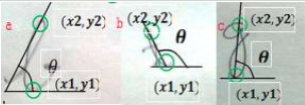
\includegraphics[width=0.85\textwidth]{figures/char_angle.png}
    \caption{Пример расчета угла наклона символа}
    \label{fig:architecture:symbol_angle}
\end{figure}

На изображении~\ref{fig:architecture:symbol_angle} приведены примеры символов с выделенными верхними и нижними точками, координаты $ (x_2, y_2) и (x_1, y_1) $ соответственно и условно обозначенным угол $ \Theta $. Представлены образцы трех типов наклона символов левосторонний, правосторонний и прямой.

Сегментация рукописного текста является нетривиальной задачей ввиду непостоянства таких параметров как пробелы между символами, в плодь до их отсутствия, словами и строками. Задача становится еще сложнее учитывая то, что данные признаки необходимо сохранить и использовать в дальнейшей работе. Так же стоит отметить что выделения силы нажатия необходимо производить до бинаризации, т.к. после бинаризации это будет невозможно.

Поскольку сегментации изображения и выделение признаков являются относительно долгими операциями, сегментация вместе с выделением признаков занимает от 0.5 до 3 секунд, в зависимости от размера изображения, обеспечение параллельной обработки выходит на передний план. К счастью выбранные признаки почерка независимы и могут рассчитываться параллельно. Так же нет необходимость ожидать полной сегментации изображения для начала выделения признаков, например интервал между строками можно вычислить сразу после разбиения изображения на строки. Это позволит значительно ускорить работу данного модуля.

\subsection{Модуль доступа к данным}
Данный модуль отвечает за организацию работы с базой данных и предоставление другим модулям удобного интерфейса.
На основании требований сформированных в разделах~\ref{sec:freq:show},~\ref{sec:freq:add},~\ref{sec:freq:delete} и~\ref{sec:freq:package_add}, основными функциями данного модуля являются:
\begin{itemize}
  \item добавление авторизационных данных пользователя в базу при регистрации (включая проверку дублирования имен пользователей);
  \item проверка наличия пользователя в базе и соответствие хеша пароля;
  \item добавление нового изображения в базу;
  \item обновление информации о параметрах изображения;
  \item удаление изображения из базы.
\end{itemize}

Так как список параметров изображения не постоянный и параметры рассчитываются и обновляются параллельно, использование классической реляционной базы данных в данном случае нерационально, в тоже время на базу данных на налагается каких-либо существенных ограничений по быстродействию и скорости обработки запросов. Основываясь на выше перечисленном в качестве СУБД была выбрана MongoDB.
Так же плюсом этого решения можно отнести хранение документов в базе в виде JSON-объектов, что исключает дополнительное преобразование данных перед отправкой их другим сервисам и на клиент, а так же отсутствие платы за использование, что позволит снизить стоимость разработки и использования.

\subsection{Модуль контроля доступа}
Поскольку разрабатываемое приложение может содержать персональные данные пользователя, вплоть до имени и фамилии в графе комментариев к изображению, задача организации безопасного доступа и хранению подобных данных стоит довольно остро.
Данный модуль отвечает за регистрацию и авторизацию пользователей. 
В данном проекте для предоставления защищенного доступа к модулям будет использоваться открытый стандарт JSON Web Token (RFC 7519). JWT-маркер  содержит в зашифрованном виде всю минимально необходимую информацию для аутентификации и авторизации. При этом не требуется хранить в сессии данных о пользователе, так как маркер самодостаточный. Данный факт упрощает горизонтальное масштабирование системы и хорошо подход для архитектур на основе микросервисов.

На основании требований, сформированных в разделах~\ref{sec:freq:reg} и~\ref{sec:freq:auth}, основными функциями данного модуля являются:
\begin{itemize}
  \item регистрации новых пользователей;
  \item авторизация пользователей;
  \item генерация JWT"=маркеров.
\end{itemize}

\begin{figure}[ht]
    \centering
    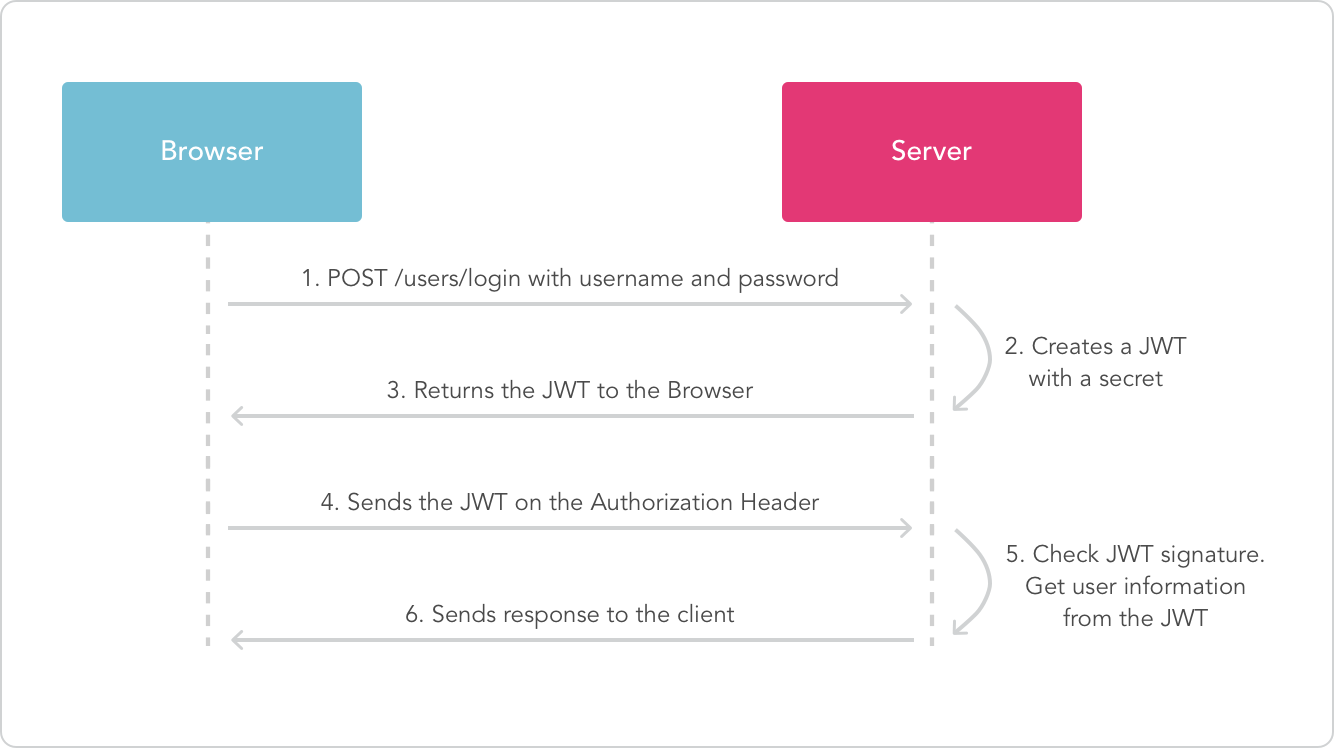
\includegraphics[width=0.7\textwidth]{figures/jwt_diagram.png}
    \caption{Диаграмма генерации и верификации JWT-маркеров}
    \label{fig:architecture:jwt_diagram}
\end{figure}

На рисунке~\ref{fig:architecture:jwt_diagram} представлен алгоритм создания, подписи и проверки JWT-маркера. В данном примере выдачу и проверку маркера осуществляет один и тот же сервер, однако, как было описано выше, это не является обязательным условием и представлено лишь для упрощения диаграммы.

Использование контроля доступа на основе JWT-маркеров позволяет снизить нагрузку на сервис контроля доступа, благодаря возможности проверки подлинности маркера на стороне других сервисов.

 %

% Глава 4 Разработка программного средства
\section{Разработка программного средства}

В данном раздела описывается процесс разработки программного \mbox{средства.}
\subsection{Обучение классификатора}
Правильная классификация черт личности является основной задачей данного проекта, результат зависит от предподготовки данных, процедуры оценки результата и финального качества обучения.

\begin{figure}[h]
    \centering
    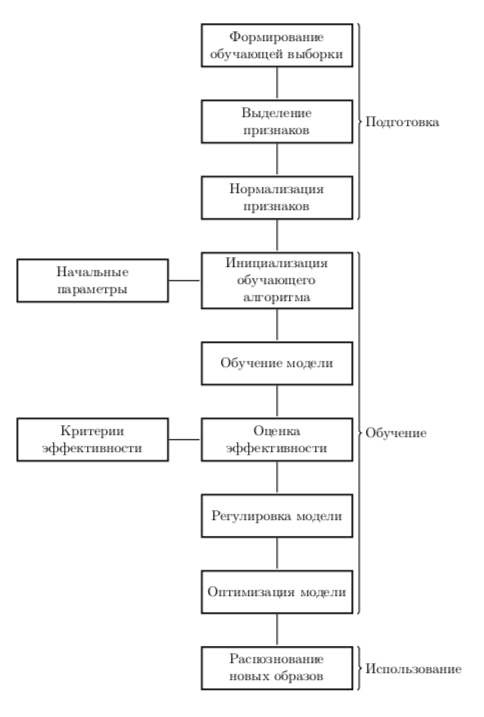
\includegraphics[width=0.7\textwidth]{figures/SVM_flow.png}
    \caption{Алгоритм обучения}
    \label{fig:develoipment:svm_flow}
\end{figure}

Общая схема подготовки, обучения и использования классификатора представлена на рисунке~\ref{fig:develoipment:svm_flow}.

После обучения классификатора можно переходить к классификации образов. В листинге~\ref{listing:development:classification} представлен метод классификации нового образца почерка на основе обученной модели. Всего в программном средстве различается 16 типов личности определяющих характеристики.

\lstinputlisting[
    style=commonstyle,
    caption=Метод классификации личности по параметрам почерка,
    label=listing:development:classification
]{src/evaluate_single_instance.java}

\todo[inline]{Все так же только образцы прошли предобработку по трансформации изображений с набор координат, отсутствующие параметры заменены значениями по умолчанию}
Для обучения классификатора будет использоваться обучающая выборка <<IAM Handwriting Database>>~\cite{IAM_handwriting_database} состоящая из 1539 образцов текста, написанных 500 авторами, с заранее выделенными параметрами почерка либо на основании выделенных параметров можно рассчитать параметры используемые в данной работе. Образцы почерка представлены изображениями в формате png, а параметры XML документом, пример параметров представлен в листинге~\ref{listing:development:sample_set}.
\lstinputlisting[
    style=commonstyle,
    caption=Пример XML-документа описывающего параметры почерка,
    label=listing:development:sample_set
]{src/sample_set.xml}

Данный объем и содержание обучающей выборки позволяет добиться хорошего качества классификации после обучения благодаря репрезентативности, в частности максимальная разность в количестве образцов разных классов составляет 13\%.
\todo[inline]{Обновить иерархию}
\subsection{Иерархия классов}
\begin{figure}[!ht]
    \centering
    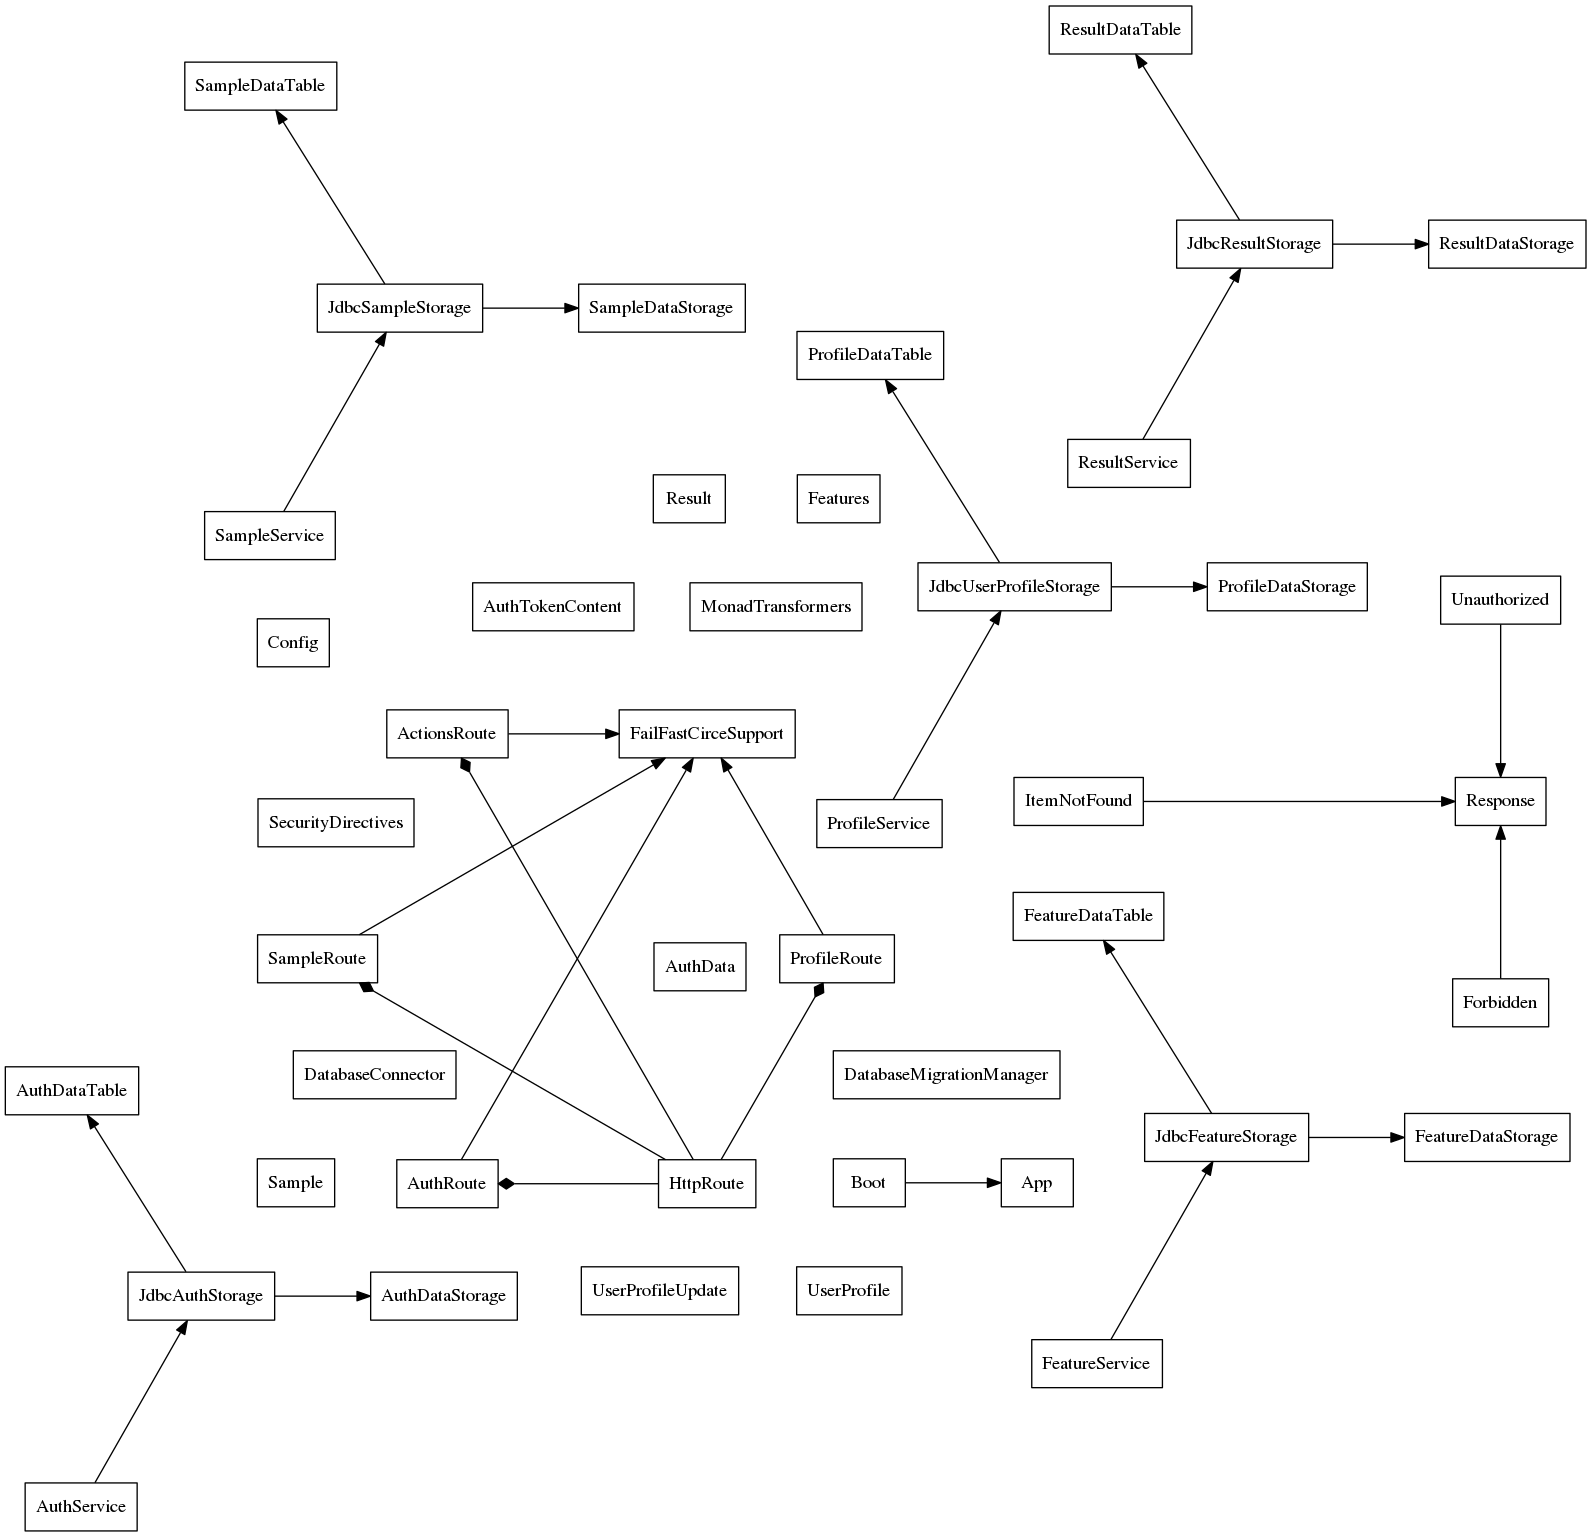
\includegraphics[width=1\textwidth]{figures/classes-fdp.png}
    \caption{Иерархия классов}
    \label{fig:develoipment:class_fdp}
\end{figure}

Общая диаграмма иерархии классов представлена на рисунке~\ref{fig:develoipment:class_fdp}. Все классы отвечающие за обработку запросов и данных, в частности \emph{ModelActor}, \emph{ParserActor}, \emph{ServiceActor} являются наследниками класса \emph{Actor} библиотека Akka. Это свидетельствует о том, что обработка информации на всех уровнях приложения происходит асинхронно.

Классы \emph{ItemNotFound}, \emph{Forbidden}, \emph{Unauthorized} являются наследниками класса \emph{Response} и представляют собой обертки для HTTP ответов на различные ошибочные ситуации на стороне клиента.

Классы \emph{ProductionTopLevel}, \emph{TopLevel} и \emph{TopLevelConfig} позволяют реализовать механизм управления зависимостями называемый \emph{Cake pattern}. При данном подходе все зависимости модуля, интерфейсы которые он использует в работе, перечисляются в специальной секции. Достоинствами данного подходя является полная поддержка средствами языка и проверка зависимостей на этапе компиляции.

Приведенная диаграмма является обобщенной диаграммой каждого модуля и представленные в ней элементы и связи справедливы для всех сервисов разработанного программного средства. Различия заключается лишь в функциях классов сервиса, например \emph{ModelActor} в сервисе доступа к базе данных отвечает за общение с базой данных, а в сервисе определения параметров личности за локальный кеш признаков образца.

Общая структура разделения кода на классы в каждом модуле позволит упростить понимания взаимодействия классов внутри всех модулей после изучения кода хотя бы одного из них.

\subsection{Маршрутизация запросов}
Библиотека Spray, описанная в пункте~\ref{sec:techs:spray}, имеет очень выразительный внутренний язык описания разбора, обработки и маршрутизации запросов к сервису. Модуль доступа к данным является связующий звеном между модулями приложения и базой данных. Поскольку одной из задач программного средства является предотвращение не авторизированного доступа к данным. Каждый обработчик запросов содержит секцию отвечающую за проверку прав доступа.
\lstinputlisting[
    style=commonstyle, 
    caption=Маршрутизация запросов к серверу в модуле доступа к данным,
    label=listing:development:db_rout
]{src/routing.scala}
Конструкция \emph{authorizeToken} описанная в модуле \emph{spray-jwt} отвечает за проверку прав доступа, подробнее будет рассмотрена в разделе~\ref{sec:development:access_control}, а \emph{path} отвечает за маршрутизацию и разбор параметров запросов. 

Использование высоко-интегрированных компонентов, таких как \emph{spray-jwt} позволяет снизить риски некорректной работы при обновлении версий одного из компонентов и ускорить разработку и сопровождения благодаря использованию схожих концепций и стиля разработки.

\subsection{Хранение данных}
Для хранения учетных и пользовательских данных используется СУБД MongoDB. Условно все данные можно разделить на образцы изображений, листинг~\ref{listing:development:json:sample} и описание пользовательских данных, листинг~\ref{listing:development:json:user}. Для хранения используется формат JSON что упрощает преобразование информации при общения сервисов между собой и с клиентом. 

\lstinputlisting[
    style=commonstyle,
    caption=Пример JSON-документа описывающего образец текста,
    label=listing:development:json:sample
]{src/sample_item.json}

\lstinputlisting[
    style=commonstyle,
    caption=Пример JSON-документа описывающего пользователя,
    label=listing:development:json:user
]{src/user_item.json}

\subsection{Контроль доступа}
\label{sec:development:access_control}
Для контроля доступа используется механизм основанный на использовании JWT-маркера. Основой данного подхода является использование асинхронной криптографии для подписи и проверки JWT-маркера и доверее информации хранящейся в нем. Для подписи используется алгоритм RSA.

В разрабатываемом программное средстве для обеспечение создания, подписи и проверки JWT-маркеров используется модуль \emph{spray-jwt}. Модуль авторизации после после сравнения имени пользователя и пароля с авторизационных данными хранящимися в базе, создает новый JWT-маркер содержащий уникальный идентификатор пользователя, алгоритм подписи, срок действия, тип маркера, а так же информацию о том является ли он администратором. Далее модуль авторизации подписывает созданный маркер своим секретным ключом и добавляет подпись к маркеру. Так же есть возможность передавать отрытый ключ для его проверки в теле маркера.
Финальное содержание JWT-маркера представлено в листинге~\ref{listing:development:jwt_token}. Далее весь маркер переводится в кодировку Base64, части маркера разделяются точкой, и прикрепляется к ответу клиента.
\lstinputlisting[
    style=commonstyle,
    caption=Пример JWT-маркера,
    label=listing:development:jwt_token
]{src/jwt_token.json}

Клиент получив JWT-маркер использует его для подтверждения прав доступа при запросам к сервисам входящим в состав программного средства прикрепляя его к запросам.

Каждый из сервисов приложения имеет открытый ключ, являющийся парным к закрытому ключу сервиса авторизации, для проверки подлинности подписи маркера. После чего данные содержащиеся в теле маркера могут быть использованы в работе, так как их подлинность доказана. Такой подход позволяет снизить нагрузку на сервис авторизации благодаря возможности сервисов самостоятельно осуществлять проверку подлинности маркера.

\subsection{Сборка и развертывание}
Для получения последнюю версию исходного кода программного средства используйте команду <<git clone>> в корневом каталоге ПС. Разрешение зависимостей, сборка и развертывание программного средства выполняется с помощью автоматической системы сборки sbt~\cite{sbt}, поэтому перед началом сборки необходимо установить данный инструмент. Программное средство в своей работе использует ряд библиотек. При помощи команды <<sbt>> в корневом каталоге ПС будет произведены загрузка всех необходимых библиотек включая компилятор языка Scala, а так же компиляция модуля программного средства.
Для развертывания модуля программного средства необходимо указать параметры развертывания в файле \emph{application.conf}, подробнее об этом рассказывается в главе~\ref{sec:manpage:admin_man}, и выполнить команду <<sbt run>>. Процесс сборки и развертывания практически полностью выполняется автоматически и не должен вызвать проблем.

Помимо этого сборка и развертывание приложения на тестовом окружении осуществляется автоматически при внесении изменений в базу исходного кода командой <<git push>>.

В данном разделе была рассмотрена общая структура обучение классификатора на основе метода опорных векторов, диаграмма иерархии классов разработанного программного средства, формата хранения внутрих данных приложения, таких как учетные записи пользователей и образцы почерка, а так же внешние данные, обучающую выборку. На данном этапе разработка и отладка программное средства закончена и можно переходи к его тестированию. %

% Глава 5 Тестирование программного средства
\section{Тестирование программного средства}
\label{sec:testing}

Разработанное программное средство представляет собой набор программных модулей и сервер базы данных. Тестирование программного средства представляет собой проверку работоспособности самих разработанных модулей независимо от сервера базы данных. 
Перед подготовки программного средства к тестированию необходимо выполнить следующие действия:
\begin{enumerate}
  \item развернуть все модули программного средства;
  \item сконфигурировать доступ к базе данных;
  \item сконфигурировать адреса сервисов выделения признаков и определения психологических характеристик в модуле распределения нагрузки.
\end{enumerate}

Для оценки правильности работы программного средства было проведено тестирование. В данном разделе приведены тест-кейсы и их результаты в вид таблиц.

\begin{longtable}[l]{| >{\raggedright}p{0.3\textwidth}
                     | >{\raggedright}p{0.3\textwidth}
                     | >{\raggedright\arraybackslash}p{0.3\textwidth}|}
  \caption{Тестирование доступа к базе данных}
  \label{table:testing:db}\\
  \endfirsthead
  \caption*{Продолжение таблицы \ref{table:testing:db}}\\
  \endhead

  \hline
       Название тест-кейса и его описание & Ожидаемый результат & Фактический результат \\
   \hline
   Получение списка образцов почерка по id пользователя (неавторизированный) \\
   1) Инициализировать объект класса Database; \\
   2) вызвать функцию Database.get с id зарегистрированного устройства в качестве параметра.
   &
   1) Объект класса Database сигнализирует об успешной инициализации; \\
   2) результатом функции является объект класса Model с параметром id, использованным в запросе.
   &
   Тест пройден \\ \hline

   Получение списка образцов почерка по id пользователя (авторизированный) \\
   1) Инициализировать объект класса Database; \\
   2) вызвать функцию Database.get с id зарегистрированного устройства в качестве параметра.
   &
   1) Объект класса Database сигнализирует об успешной инициализации; \\
   2) результатом функции является объект класса Model с параметром id, использованным в запросе.
   &
   Тест пройден \\ \hline

\end{longtable}

\begin{longtable}[l]{| >{\raggedright}p{0.3\textwidth}
                     | >{\raggedright}p{0.3\textwidth}
                     | >{\raggedright\arraybackslash}p{0.3\textwidth}|}
  \caption{Тестирование модуля контроля доступа}
  \label{table:testing:bayes}\\
  \endfirsthead
  \caption*{Продолжение таблицы \ref{table:testing:bayes}}\\
  \endhead

  \hline
       Название тест-кейса и его описание & Ожидаемый результат & Фактический результат \\
   \hline
   Авторизация пользователя с неверным логином и паролем \\
   1) В интерфейсе коммандной строки набрать путь исполняемого файла и путём к файлу данных; \\
   2) нажать клавишу ввода и ожидать завершения программы.
   &
   1) Имя исполняемого модуля и путь к файлу отображаются в консоли; \\
   2) отображается результат обучения модели в виде вектора апостериорных вероятностей.
   &
   Тест пройден \\ \hline

   Авторизация пользователя с неверным логином и верным паролем \\ 
   1) В интерфейсе коммандной строки набрать путь исполняемого файла модуля с путём к файлу векторов данных и числом попыток обучения модели в качестве аргументов; \\
   2) нажать клавишу ввода и ожидать завершения программы.
   &
   1) Имя исполняемого модуля, путь к файлу и число попыток обучения отображаются в консоли; \\
   2) отображаются обученные модели в количестве, равном числу попыток, и отмечается модель с наименьшим процентом ошибок.
   &
   Тест пройден \\ \hline

   Авторизация пользователя с верным логином и паролем \\ 
   1) В интерфейсе коммандной строки набрать путь исполняемого файла модуля с путём к файлу векторов данных и числом попыток обучения модели в качестве аргументов; \\
   2) нажать клавишу ввода и ожидать завершения программы.
   &
   1) Имя исполняемого модуля, путь к файлу и число попыток обучения отображаются в консоли; \\
   2) отображаются обученные модели в количестве, равном числу попыток, и отмечается модель с наименьшим процентом ошибок.
   &
   Тест пройден \\ \hline
\end{longtable}

Далее тестируется запуск сервера с заданной конфигурацией? котороя может быть представлена в виде ini-файла или с описана с помощью перемеженных окружения.
\clearpage

\begin{longtable}[l]{| >{\raggedright}p{0.3\textwidth}
                     | >{\raggedright}p{0.3\textwidth}
                     | >{\raggedright\arraybackslash}p{0.3\textwidth}|}
  \caption{Тестирование программы построения компактной модели PUF}
  \label{table:testing:servercfg}\\
  \endfirsthead
  \caption*{Продолжение таблицы \ref{table:testing:servercfg}}\\

  \hline
       Название тест-кейса и его описание & Ожидаемый результат & Фактический результат \\
  \endhead
   \hline
   Запуск сервера с настройками по умолчанию \\
   1) В коммандной строки набрать команду запуска сервера; \\
   2) нажать клавишу ввода.
   &
   1) Имя скрипта запуска сервера отображаются в консоли; \\
   2) отображается диагностическая информация о запуске сервера и предустановленных параметра функционирования.
   &
   Тест пройден \\ \hline

   Запуск сервера с настройками из ini-файла \\
   1) В коммандной строки набрать команду запуска сервера и путь к ini-файлу в качестве аргумента; \\
   2) нажать клавишу ввода.
   &
   1) Имя скрипта запуска сервера отображаются в консоли; \\
   2) отображается диагностическая информация о запуске сервера и параметра функционирования, взятых из преоставленного ini-файла.
   &
   Тест пройден \\ \hline
\end{longtable}

\clearpage
\begin{longtable}[l]{| >{\raggedright}p{0.3\textwidth}
                     | >{\raggedright}p{0.3\textwidth}
                     | >{\raggedright\arraybackslash}p{0.3\textwidth}|}
  \caption{Тестирование взаимодействия с уcтройством}
  \label{table:testing:pufbit}\\
  \endfirsthead
  \caption*{Продолжение таблицы \ref{table:testing:pufbit}}\\
  \endhead

  \hline
       Название тест-кейса и его описание & Ожидаемый результат & Фактический результат \\
   \hline
   Использование функции PUF для получения выходного бита \\
   1) Инициировать экземпляр класса Prover c объектом Device в качестве аргумента; \\
   2) сгенерировать случайный объект Challenge с помощью объекта Prover; \\
   3) запустить функцию Device.f с аргументом Challenge.
   &
   1) Объект класса Prover возвращает статус успешной инициализации; \\
   2) объект Challenge является битовой строкой из случайных нулей и единиц; \\
   3) значением функции является случайный бит 0 или 1.
   &
   Тест пройден \\ \hline

   Использование модели функции PUF для получения выходного бита \\
   1) Инициировать экземпляр класса Verifier c объектом Device в качестве аргумента; \\
   2) сгенерировать случайный объект Challenge с помощью объекта Verifier; \\
   3) запустить функцию Model.f с аргументом Challenge.
   &
   1) Объект класса Verifier возвращае статус успешной инициализации; \\
   2) объект Challenge является битовой строкой из случайных нулей и единиц; \\
   3) значением функции является случайный бит 0 или 1.
   &
   Тест пройден \\ \hline

   \hline
\end{longtable}

\clearpage

В следующих таблицах(\ref{table:testing:proto} и \ref{table:testing:regpuf}) тестируются два основных режима: режим регистрации и режим аутенификации, при тестировании которого проверятся также случай, когда злоумышленником прелпринимается попытка аутентификации с помощью поддельного PUF. Даже случае подмены идентификатора устройства решение о предоставлении доступа будет принято на основе соответствия поведения устройства поведению зарегистрированной модели.


\begin{longtable}[l]{| >{\raggedright}p{0.3\textwidth}
                     | >{\raggedright}p{0.3\textwidth}
                     | >{\raggedright\arraybackslash}p{0.3\textwidth}|}
  \caption{Тестирование протокола аутентификации}
  \label{table:testing:proto}\\
    \hline
       Название тест-кейса и его описание & Ожидаемый результат & Фактический результат \\
    \hline
  \endfirsthead
  \caption*{Продолжение таблицы \ref{table:testing:proto}}\\

  \hline
       Название тест-кейса и его описание & Ожидаемый результат & Фактический результат \\
   \hline
  \endhead
  \endlastfoot
   Аутентификация незарегистрированного устройства \\
   1) Инициировать объект класса Device, связанного с незарегистрированным устройством; \\
   2) подменить поле id объекта Device, на id, связанный с зарегистрированным устройством; \\
   3) инициировать экземпляр класса Prover c объектом Device и адресом сервера аутентификации в качестве аргументов; \\
   4) вызвать функцию Prover.authenticate.
   &
   1) Объект класса Device имеет id незарегистрированного устройства; \\
   2) объект класса Device имеет id зарегистрированного устройства; \\
   3) объект класса Prover возвращает статус успешной инициализации; \\
   4) сервер возвращает сообщение об отклонение запроса и предупреждение о поддельном устройстве.
   &
   Тест пройден \\

   Аутентификация подлинного устройства \\
   1) Инициировать объект класса Device, связанного с зарегистрированным устройством; \\
   2) инициировать экземпляр класса Prover c объектом Device и адресом сервера аутентификации в качестве аргументов; \\
   3) вызвать функцию Prover.authenticate.
   &
   1) Объект класса Device имеет id зарегистрированного устройства; \\
   2) объект класса Prover возвращает статус успешной инициализации; \\
   3) сервер возвращает сообщение об успешной аутентификации.
   &
   Тест пройден \\
   \hline


\end{longtable}


\begin{longtable}[l]{| >{\raggedright}p{0.3\textwidth}
                     | >{\raggedright}p{0.3\textwidth}
                     | >{\raggedright\arraybackslash}p{0.3\textwidth}|}
  \caption{Тестирование регистрации устройства}
  \label{table:testing:regpuf}\\
  \endfirsthead
  \caption*{Продолжение таблицы \ref{table:testing:regpuf}}\\
  \endhead

  \hline
       Название тест-кейса и его описание & Ожидаемый результат & Фактический результат \\
   \hline
   Регистрация устройства в базе данных \\
   1) Инициировать экземпляр класса Prover c объектом Device в качестве аргумента; \\
   2) вызвать функцию Prover.register. \\
   &
   1) Объект класса Prover возвращает статус успешной инициализации; \\
   2) сервер возвращает сообщение об успешной регистрации.
   &
   Тест пройден \\ \hline
\end{longtable}
 %

% Глава 6 Использование разработанного программного средства
\section{Методика использования программного средства}
\label{sec:manpage}

Программное средство определения параметров личности по анализу образцов почерка работает как веб-приложение. Ниже приведено описание вариантов использования и конфигурации модулей приложения.

\subsection{Руководство администратора}
\label{sec:manpage:admin_man}
Модули разрабатываемого программного средства разворачиваются как независимые компоненты, что позволяет добиться большой гибкости.

Конфигурация модулей осуществятся с помощью файла \emph{application.conf} расположенного в папке \emph{resources} в каталоге с файлами модуля. Для описания конфигурации используется формат HOCON позволяющий представить конфигурацию в легко-читаемом форме. 

\lstinputlisting[
    style=commonstyle,
    caption=Пример файла конфигурации модуля,
    label=lst:manpage:app_conf
]{src/application.conf}

Варьируя параметры \emph{host} и \emph{port} можно добиться развертывания модуля на произвольном адресе.

Помимо параметров развертывания и адресов других модулей файл конфигурации модуля доступа к данным содержит блок отвечающий за информацию о базе данных.

\lstinputlisting[
    style=commonstyle,
    caption=Пример блока конфигурации доступа к базе данных,
    label=lst:manpage:db_conf
]{src/mongodb.conf}

Наиболее важными параметрами являются \emph{connection-string}, \emph{user-name} и \emph{password}. С помощью параметра \emph{connection-string} указывается адрес сервера баз данных и имя базы, а параметра \emph{user-name} и \emph{password} отвечают за авторизационные данные. Так же при низкой скорость интернет соединения может возникнуть необходимость увеличить значение параметра \emph{connection-timeout}. 

\subsection{Руководство пользователя}
\label{sec:manpage:client_man}
Данный раздел содержит инструкции по использованию основных возможностей программного средства и позволят конечным пользователям быстрее научиться эффективно взаимодействовать с ним. %

% Глава 7 Технико-экономическое обоснование разработки ПС
\def \byr{Br}

\section{Технико-экономическое обоснование разработки ПС}

% Категория сложности
\def \complexityGroup{3}

% Категория новизны
\def \noveltyGroup{Б}

% ---

Целью дипломного проектирования является создание программного средства для распознавания уникальных идентификаторов цифровых устройств с целью их аутентификации. Данное ПС реализует протокол аутентификации на основе использования и анализа информации, полученной от специального компонента цифрового устройства, выполненного в виде физически неклонируемой функции (ФНФ). Основными достоинствами программного средства являются: высокая производительность при низких системных требованиях; модульная архитектура, разделяющая взаимодействие с устройством, обработку идентификационных данных и аутентификацию.

В данном разделе рассмотрим экономическую эффективность программного средства. Программный комплекс относится к \complexityGroup-й группе сложности. Категория новизны продукта – <<\noveltyGroup>>. Для оценки экономической эффективности ПС необходимо рассчитать смету затрат на разработку, цену и прибыль продажи одной программной системы.

Расчеты выполнены на основе методического пособия~\cite{palicyn_2006}.



\subsection{Расчёт сметы затрат и цены программного продукта}

% Коэффициент сложности, ед.
\def \additionalComplexityFactor{0.12}
\FPeval{complexityFactor}{clip(1 + \additionalComplexityFactor)}

% Степень использования при разработке стандартных модулей, ед.
\def \stdModuleUsageFactor{0.6}

% Коэффициент новизны, Кн
\def \noveltyFactor{0.9}

% Годовой эффективный фонд времени, дн.
\def \daysInYear{366}
\def \holidaysInYear{6}
\def \weekendDaysInYear{105}
\def \vacationDaysInYear{24}
\FPeval{workingDaysInYear}{
    clip(\daysInYear -
         \holidaysInYear -
         \weekendDaysInYear -
         \vacationDaysInYear)
}

% Среднемесячная норма рабочего времени, Фр
\def \workingHoursInMonth{160}

% Продолжительность рабочего дня, ч.
\def \workingHoursInDay{8}

% Месячная тарифная ставка первого разряда, Br
% \def \tariffRate{298000} % Гос. предприятия
\def \tariffRate{1150000}

% Коэффициент премирования, ед
\def \bonusRate{1.5}

% Норматив дополнительной заработной платы, Br
\def \additionalSalaryRate{20}

% Норматив отчислений в ФСЗН и обязательное страхование, %
\def \socialProtectionRate{34}

% Норматив отчислений в Белгосстрах
\def \bgsRate{0.7}

% Норматив командировочных расходов, %
\def \businessTripRate{15}

% Норматив прочих затрат, %
\def \otherExpenseRate{20}

% Норматив накладных расходов, %
\def \overheadExpenseRate{100}

% Прогнозируемый уровень рентабельности, %
\def \profitability{35}

% Норматив отчислений в местный и республиканский ю.джет
\def \localRepubTaxRate{3.9}

% Норматив НДС, %
\def \vatRate{20}

% Норматив налога на прибыль, %
\def \profitTaxRate{18}

% Норматив расхода материалов, %
\def \materialsRate{3}

% Норматив расхода машинного времени, ч.
\def \debugRate{15} % часов / 100 строк кода

% Цена одного часа машинного времени, Br
\def \machineHourCost{25000}

% Норматив расходов на сопровождение и адаптацию ПО, %
\def \supportAndAdaptationRate{30}

% ---
На основании сметы затрат и анализа рынка ПО определяется плановая отпускаемая цена.
Для составления сметы затрат на создание ПО необходима предварительная оценка трудоемкости ПО и его объёма.
Расчет объёма программного продукта предполагает определение типа программного обеспечения, всестороннее техническое обоснование функций ПО и определение объёма каждой функций.
Согласно классификации типов программного обеспечения~\cite[с.~59,~приложение 1]{palicyn_2006}, разрабатываемое ПО можно классифицировать как ПО методo"=ориентированных расчетов.

Исходные данные разрабатываемого проекта указаны в таблице~\ref{table:economics:initial_data}.
\afterpage{
\begin{longtable}[l]{| >{\raggedright}m{0.62\textwidth}
                     | >{\centering}m{0.17\textwidth}
                     | >{\centering\arraybackslash}m{0.13\textwidth}|}

    \caption{Исходные данные}
    \label{table:economics:initial_data}
    \\

    \hline
    {\begin{center} Наименование \end{center} } & Условное обозначение & Значение
    \\ \hline

    Категория сложности
    & & \complexityGroup
    \\ \hline

    Коэффициент сложности, ед.
    & $ \text{К}_\text{с} $ & \num{\complexityFactor}
    \\ \hline

    Степень использования при разработке стандартных модулей, ед.
    & $ \text{К}_\text{т} $ & \num{\stdModuleUsageFactor}
    \\ \hline

    Коэффициент новизны, ед.
    & $ \text{К}_\text{н} $ & \num{\noveltyFactor}
    \\ \hline

    Годовой эффективный фонд времени, дн.
    & $ \text{Ф}_\text{эф} $ & \num{\workingDaysInYear}
    \\ \hline

    Продолжительность рабочего дня, ч.
    & $ \text{Т}_\text{ч} $ & \num{\workingHoursInDay}
    \\ \hline

    Месячная тарифная ставка первого разряда, \byr{}
    & $ \text{Т}_{\text{м}_{1}}$ & \num{\tariffRate}
    \\ \hline

    Коэффициент премирования, ед.
    & $ \text{К} $ & \num{\bonusRate}
    \\ \hline

    Норматив дополнительной заработной платы, ед.
    & $ \text{Н}_\text{д} $ & \num{\additionalSalaryRate}
    \\ \hline

    Норматив отчислений в ФСЗН, $\%$
    & $ \text{Н}_\text{сз} $ & \num{\socialProtectionRate}
    \\ \hline

    Норматив отчислений в Белгосстрах, $\%$
    & $ \text{Н}_\text{с} $ & \num{\socialProtectionRate}
    \\ \hline

    Норматив командировочных расходов, $\%$
    & $ \text{Н}_\text{к} $ & \num{\businessTripRate}
    \\ \hline

    Норматив прочих затрат, $\%$
    & $ \text{Н}_\text{пз} $ & \num{\otherExpenseRate}
    \\ \hline

    Норматив накладных расходов, $\%$
    & $ \text{Н}_\text{рн} $ & \num{\overheadExpenseRate}
    \\ \hline

    Прогнозируемый уровень рентабельности,
    $\%$ & $ \text{У}_\text{рп} $ & \num{\profitability}
    \\ \hline

    Норматив НДС, $\%$
    & $ \text{Н}_\text{дс} $ & \num{\vatRate}
    \\ \hline

    Норматив налога на прибыль, $\%$
    & $ \text{Н}_\text{п} $ & \num{\profitTaxRate}
    \\ \hline

    Норматив расхода материалов, $\%$
    & $ \text{Н}_\text{мз} $ & \num{\materialsRate}
    \\ \hline

    Норматив расхода машинного времени, ч.
    & $ \text{Н}_\text{мв} $ & \num{\debugRate}
    \\ \hline

    Цена одного часа машинного времени, \byr{}
    & $ \text{Н}_\text{мв} $ & \num{\machineHourCost}
    \\ \hline

    Норматив расходов на сопровождение и адаптацию ПО, $\%$
    & $ \text{Н}_\text{рса} $ & \num{\supportAndAdaptationRate}
    \\ \hline
\end{longtable}
}

Общий объём программного продукта определяется исходя из количества и объёма функций, реализованных в программе:
\begin{equation}
  \label{eq:economics:total_loc}
  V_{o} = \sum_{i = 1}^{n} V_{i} \text{\,,}
\end{equation}
\begin{explanation}
где & $ V_{i} $ & объём отдельной функции ПО, LoC; \\
    & $ n $ & общее число функций.
\end{explanation}

На стадии технико-экономического обоснования проекта рассчитать точный объём функций невозможно.
Вместо вычисления точного объёма функций применяются приблизительные оценки на основе данных по аналогичным проектам или по нормативам~\cite[с.~61,~приложение 2]{palicyn_2006}, которые приняты в организации.

\def \totalLOC{9710} % TODO
\def \totalLOCCorrected{6390} % TODO

\afterpage{
\begin{longtable}{| >{\centering}m{0.12\textwidth}
                  | >{\raggedright}m{0.40\textwidth}
                  | >{\centering}m{0.18\textwidth}
                  | >{\centering\arraybackslash}m{0.18\textwidth}|}
  \caption{Перечень и объём функций программного модуля}
  \label{table:econ:function_sizes}
  \\

  \hline
    \multirow{2}{0.12\textwidth}[-0.5em]{\centering \No{} функции}
    & \multirow{2}{0.40\textwidth}[-0.55em]{\centering Наименование (содержание)}
    & \multicolumn{2}{c|}{\centering Объём функции, LoC} \tabularnewline

  \cline{3-4} &
       & { по каталогу ($ V_{i} $) }
       & { уточненный ($ V_{i}^{\text{у}} $) } \tabularnewline
  \hline

  101 & Организация системы подключаемых модулей
  & \num{720} & \num{520}
  \\ \hline

  102 & Контроль, предварительная обработка и ввод информации
  & \num{650} & \num{370}
  \\ \hline

  111 & Обработка исходных данных и тренировка математической модели
  & \num{3100} & \num{1900}
  \\ \hline

  301 & Интерфейс к базе данных моделей устройств
  & \num{890} & \num{770}
  \\ \hline

  501 & Монитор ПО (управление работой компонентов)
  & \num{1240} & \num{910}
  \\ \hline

  506 & Обработка исключительных ситуаций
  & \num{620} & \num{400}
  \\ \hline

  507 & Обеспечение интерфейса между компонентами
  & \num{970} & \num{680}
  \\ \hline

  612 & Аутентификация на основе сравнения реальных данных и математической модели
  & \num{1100} & \num{840}
  \\ \hline

  Итог & &
  {\num{\totalLOC}} & {\num{\totalLOCCorrected}}
  \\ \hline

\end{longtable}
}

Перечень и объём функций программного модуля перечислен в таблице~\ref{table:econ:function_sizes}.
По приведенным данным уточненный объём некоторых функций изменился, и общий уточненный объём ПО
$ V_{\text{у}} = \SI{\totalLOCCorrected}{\text{LoC}} $
.



\subsection{Расчёт трудоемкости}

% Нормативная трудоёмкость, Тн
\def \normativeWorkload{144}

% Общая трудоёмкость, То
\FPeval{totalWorkload}{
    trunc(\normativeWorkload *
          \complexityFactor *
          \stdModuleUsageFactor *
          \noveltyFactor + 0.5, 0)
}

% Срок разработки проекта, Тр
\def \developmentMonths{3}
\FPeval{developmentYears}{round(\developmentMonths / 12, 2)}

% Численность исполнителей, Чр
\FPeval{requiredProgrammers}{trunc(\totalWorkload / (\developmentYears * \workingDaysInYear) + 0.5, 0) }

% Считаем, что работы каждому достаётся поровну.
\FPeval{workloadSenior}{trunc( \totalWorkload / \requiredProgrammers, 0 )}
\FPeval{workloadLead}{clip(\totalWorkload - \workloadSenior)}

% ---

На основании общего объема ПО определяется нормативная трудоемкость (
$ \text{Т}_\text{н}$
) с учетом сложности ПО. Для ПО \complexityGroup-ой группы сложности, к которой относится разрабатываемый программный продукт, нормативная трудоемкость составит~
$ \text{Т}_\text{н} = \SI{\normativeWorkload}{\text{чел.} / \text{дн.}} $

Нормативная трудоемкость служит основой для оценки общей трудоемкости~
$ \text{Т}_\text{о} $
.
Используем формулу (\ref{eq:economics:total_workload}) для оценки общей трудоемкости для небольших проектов:
\begin{equation}
  \label{eq:economics:total_workload}
  \text{Т}_\text{о} = \text{Т}_\text{н} \cdot
                      \text{К}_\text{с} \cdot
                      \text{К}_\text{т} \cdot
                      \text{К}_\text{н} \text{\,,}
\end{equation}
\begin{explanation}
где & $ \text{К}_\text{с} $ & коэффициент, учитывающий сложность ПО; \\
    & $ \text{К}_\text{т} $ & поправочный коэффициент, учитывающий степень использования при разработке стандартных модулей; \\
    & $ \text{К}_\text{н} $ & коэффициент, учитывающий степень новизны ПО.
\end{explanation}

Дополнительные затраты труда на разработку ПО учитываются через коэффициент сложности, который вычисляется по формуле
\begin{equation}
\label{eq:economics:additional_complexity_factor}
  \text{К}_{\text{с}} = 1 + \sum_{i = 1}^n \text{К}_{i} \text{\,,}
\end{equation}
\begin{explanation}
где & $ \text{К}_{i} $ & коэффициент, соответствующий степени повышения сложности ПО за счет конкретной характеристики; \\
    & $ n $ & количество учитываемых характеристик.
\end{explanation}

Наличие двух характеристик сложности позволяет~\cite[c.~66, приложение~4, таблица~П.4.2]{palicyn_2006} вычислить коэффициент сложности
\begin{equation}
\label{eq:economics:complexity_factor}
  \text{К}_{\text{с}} = \num{1} + \num{\additionalComplexityFactor} = \num{\complexityFactor} \text{\,.}
\end{equation}

Разрабатываемое ПО использует стандартные компоненты. Согласно справочным данным~\cite[c.~68,~приложение~4, таблица~П.4.5]{palicyn_2006} коэффициент использования стандартных модулей
$ \text{К}_\text{т} = \num{\stdModuleUsageFactor} $
.

Согласно справочным данным~\cite[c.~67, приложение~4, таблица~П.4.4]{palicyn_2006}, коэффициент новизны для разрабатываемого ПО
$ \text{К}_\text{н} = \num{\noveltyFactor} $
.

Подставив приведенные выше коэффициенты для разрабатываемого ПО в формулу~(\ref{eq:economics:total_workload}) получим общую трудоемкость разработки
\begin{equation}
  \label{eq:economics:total_workload_calc}
  \text{Т}_\text{о} = \num{\normativeWorkload}
                      \cdot \num{\complexityFactor}
                      \cdot \num{\stdModuleUsageFactor}
                      \cdot \num{\noveltyFactor}
                    \approx \SI{\totalWorkload}{\text{чел.}/\text{дн.}}
\end{equation}

На основе общей трудоемкости и требуемых сроков реализации проекта вычисляется плановое количество исполнителей.
Численность исполнителей проекта рассчитывается по формуле:
\begin{equation}
  \label{eq:economics:num_of_programmers}
  \text{Ч}_\text{р} = \frac{\text{Т}_\text{о}}
                           {\text{Т}_\text{р}
                      \cdot \text{Ф}_\text{эф}} \text{\,,}
\end{equation}
\begin{explanation}
где & $ \text{Т}_\text{о} $ & общая трудоемкость разработки проекта, $ \text{чел.}/\text{дн.} $; \\
    & $ \text{Ф}_\text{эф} $ & эффективный фонд времени работы одного работника в течение года, дн.; \\
    & $ \text{Т}_\text{р} $ & срок разработки проекта, лет.
\end{explanation}

Эффективный фонд времени работы одного разработчика вычисляется по формуле
\begin{equation}
  \label{eq:economics:workload_per_programmer}
  \text{Ф}_\text{эф} = \text{Д}_\text{г} -
                       \text{Д}_\text{п} -
                       \text{Д}_\text{в} -
                       \text{Д}_\text{о} \text{\,,}
\end{equation}
\begin{explanation}
где & $ \text{Д}_\text{г} $ & количество дней в году, дн.; \\
    & $ \text{Д}_\text{п} $ & количество праздничных дней в году, не совпадающих с выходными днями, дн.; \\
    & $ \text{Д}_\text{в} $ & количество выходных дней в году, дн.; \\
    & $ \text{Д}_\text{п} $ & количество дней отпуска, дн.
\end{explanation}

Согласно данным, приведенным в производственном календаре для пятидневной рабочей недели в 2017 году для Беларуси~\cite{belcalendar_2017}, фонд рабочего времени составит
\begin{equation}
  \text{Ф}_\text{эф} = \num{\daysInYear} -
                       \num{\holidaysInYear} -
                       \num{\weekendDaysInYear} -
                       \num{\vacationDaysInYear}
                     = \SI{\workingDaysInYear}{\text{дн.}}
\end{equation}

Учитывая срок разработки проекта
$ \text{Т}_\text{р} = \SI{\developmentMonths}{\text{мес.}} = \SI{\developmentYears}{\text{года}} $
, общую трудоемкость и фонд эффективного времени одного работника, вычисленные ранее, можем рассчитать численность исполнителей проекта
\begin{equation}
  \label{eq:econ:num_of_programmers_calc}
  \text{Ч}_\text{р} = \frac{\num{\totalWorkload}}
                           {\num{\developmentYears}
                      \cdot \num{\workingDaysInYear}}
                    \approx \SI{\requiredProgrammers}{\text{рабочих}}.
\end{equation}

Вычисленные оценки показывают, что для выполнения запланированного проекта в указанные сроки необходимо \requiredProgrammers ~рабочих.



\subsection{Расчёт заработной платы исполнителей}

% Тариффные коэффициенты, Тк
\def \tariffFactorSenior{3.25} % == 14 разряд
\def \tariffFactorLead{3.48}   % == 15 разряд

% Часовая тарифная ставка исполнителей, Тч
\FPeval{hourlySalarySenior}{round( \tariffRate * \tariffFactorSenior / \workingHoursInMonth, 0 )}
\FPeval{hourlySalaryLead}{round( \tariffRate * \tariffFactorLead / \workingHoursInMonth, 0 )}

% Основная арплата, Зо
\FPeval{baseSalary}{
     round(\workingHoursInDay *
           \bonusRate *
           (\hourlySalarySenior * \workloadSenior +
            \hourlySalaryLead * \workloadLead), 0)
}

% Дополнительная зарплата, Зд
\FPeval{additionalSalary}{ round( \baseSalary * \additionalSalaryRate / 100, 0 ) }


% ---

Информация о работниках перечислена в таблице~\ref{table:economics:programmers}.
\begin{table}[ht]
  \caption{Работники, занятые в проекте}
  \label{table:economics:programmers}
  \begin{tabular}{| >{\centering}m{0.4\textwidth}
                  | >{\centering}m{0.15\textwidth}
                  | >{\centering}m{0.18\textwidth}
                  | >{\centering\arraybackslash}m{0.15\textwidth}|}
   \hline
   Исполнители & Разряд & Тарифный коэффициент & \mbox{Чел./дн.} занятости
   \\ \hline

   Программист \Rmnum{1}-категории & $ \num{14} $ & $ \num{\tariffFactorSenior} $ & $ \num{\workloadSenior} $
   \\ \hline
   Ведущий программист & $ \num{15} $ & $ \num{\tariffFactorLead} $ & $ \num{\workloadLead} $
   \\ \hline
  \end{tabular}
\end{table}

Месячная тарифная ставка одного работника вычисляется по формуле
\begin{equation}
  \label{eq:economics:monthly_salary}
  \text{Т}_\text{ч} =
    \frac {\text{Т}_{\text{м}_{1}} \cdot \text{Т}_{\text{к}} }
          {\text{Ф}_{\text{р}} }  \text{\,,}
\end{equation}
\begin{explanation}
где & $ \text{Т}_{\text{м}_{1}} $ & месячная тарифная ставка 1-го разряда, \byr; \\
    & $ \text{Т}_{\text{к}} $ & тарифный коэффициент, соответствующий установленному тарифному разряду; \\
    & $ \text{Ф}_{\text{р}} $ & среднемесячная норма рабочего времени, час.
\end{explanation}

Подставив данные из таблицы~\ref{table:economics:programmers} в формулу~(\ref{eq:economics:monthly_salary}), приняв значение тарифной ставки 1-го разряда
$ \text{Т}_{\text{м}_{1}} = \SI{\tariffRate}{\text{\byr}} $
и среднемесячную норму рабочего времени
$ \text{Ф}_{\text{р}} = \SI{\workingHoursInMonth}{\text{часов}} $
получаем
\begin{equation}
  \label{eq:economics:monthly_salary_senior}
  \text{Т}_{\text{ч}}^{\text{прогр. \Rmnum{1}-разр.}} =
      \frac{ \num{\tariffRate} \cdot \num{\tariffFactorSenior} }
           { \num{\workingHoursInMonth} }
    = \SI{\hourlySalarySenior}{\text{\byr}/\text{час;}}
\end{equation}
\begin{equation}
  \label{eq:economics:monthly_salary_lead}
  \text{Т}_{\text{ч}}^{\text{вед. прогр.}} =
      \frac{ \num{\tariffRate} \cdot \num{\tariffFactorLead} }
           { \num{\workingHoursInMonth} }
    = \SI{\hourlySalaryLead}{\text{\byr}/\text{час.}}
\end{equation}

Основная заработная плата исполнителей на конкретное ПО рассчитывается по формуле
\begin{equation}
  \label{eq:economics:base_salary}
  \text{З}_{\text{о}} = \sum^{n}_{i = 1}
                        \text{Т}_{\text{ч}}^{i} \cdot
                        \text{Т}_{\text{ч}} \cdot
                        \text{Ф}_{\text{п}} \cdot
                        \text{К}
                        \text{\,,}
\end{equation}
\begin{explanation}
где & $ \text{Т}_{\text{ч}}^{i} $ & часовая тарифная ставка \mbox{$ i $-го} исполнителя, \byr$/$час; \\
    & $ \text{Т}_{\text{ч}} $ & количество часов работы в день, час; \\
    & $ \text{Ф}_{\text{п}} $ & плановый фонд рабочего времени \mbox{$ i $-го} исполнителя, дн.; \\
    & $ \text{К} $ & коэффициент премирования.
\end{explanation}

Подставив ранее вычисленные значения и данные из таблицы~\ref{table:economics:programmers} в формулу~(\ref{eq:economics:base_salary}) и приняв коэффициент премирования
$ \text{К} = \num{\bonusRate} $
получим
\begin{equation}
  \label{eq:economics:base_salary_calc}
  \text{З}_{\text{о}} = (\hourlySalarySenior \cdot \num{\workloadSenior} +
                         \hourlySalaryLead \cdot \num{\workloadLead})
                        \cdot \num{\workingHoursInDay}
                        \cdot \num{\bonusRate}
                      = \SI{\baseSalary}{\text{\byr}} \text{\,.}
\end{equation}

Дополнительная заработная плата включает выплаты предусмотренные законодательством от труде и определяется по нормативу в процентах от основной заработной платы
\begin{equation}
  \label{eq:economics:additional_salary}
  \text{З}_{\text{д}} =
    \frac {\text{З}_{\text{о}} \cdot \text{Н}_{\text{д}}}
          {100\%} \text{\,,}
\end{equation}
\begin{explanation}
  где & $ \text{Н}_{\text{д}} $ & норматив дополнительной заработной платы, $ \% $.
\end{explanation}

Приняв норматив дополнительной заработной платы
$ \text{Н}_{\text{д}} = \num{\additionalSalaryRate\%} $
и подставив известные данные в формулу~(\ref{eq:economics:additional_salary}) получим
\begin{equation}
  \label{eq:econ:additional_salary_calc}
  \text{З}_{\text{д}} =
    \frac{\num{\baseSalary} \cdot 20\%}
         {100\%} \approx \SI{\additionalSalary}{\text{\byr}} \text{\,.}
\end{equation}


\clearpage % Hack

\subsection{Расчёт расходов и прогнозируемой цены ПО}

\FPeval{totalSalary}{\baseSalary + \additionalSalary}

% Отчисления в фонд социальной защиты
\FPeval{socialProtectionMoney}{ round( \totalSalary * \socialProtectionRate / 100, 0 ) }

% Отчисления в белгосстрах
\FPeval{bgsMoney}{ round( \totalSalary * \bgsRate / 100, 0 ) }

% Материалы и комплектующие
\FPeval{materialsMoney}{ round( \baseSalary * \materialsRate / 100, 0 ) }

% Машинное время
\FPeval{machineTimeMoney}{
    round(\machineHourCost *
          \totalLOCCorrected *
          \debugRate / 100, 0)
}

% Расходы на научные командировки
\FPeval{businessTripMoney}{ round( \baseSalary * \businessTripRate / 100, 0 ) }

% Прочие прямые расходы
\FPeval{otherExpenseMoney}{ round( \baseSalary * \otherExpenseRate / 100, 0 )}

% Накладные расходы
\FPeval{overheadExpenseMoney}{ clip(round( \baseSalary * \overheadExpenseRate / 100, 0 ))}

% Общая сумма
\FPeval{\totalExpense}{
    round( \totalSalary +
           \additionalSalary +
           \socialProtectionMoney +
           \materialsMoney +
           \machineTimeMoney +
           \businessTripMoney +
           \otherExpenseMoney +
           \overheadExpenseMoney, 0 )
}

% Сопровождение и адаптация ПО
\FPeval{supportAndAdaptationMoney} { round( \totalExpense * \supportAndAdaptationRate / 100, 0 )}

% Полная себестоимость ПО
\FPeval{totalSoftwareCost}{ clip(\totalExpense + \supportAndAdaptationMoney) }

% Прогнозируемая прибыль
\FPeval{profitMoney}{ round( \totalSoftwareCost * \profitability / 100, 0) }

% Прогнозируемая цена без налогов
\FPeval{estimatedPrice}{clip( \profitMoney + \totalSoftwareCost )}

% Отчисления и налоги в местный и республиканский бюджеты
\FPeval{localRepubTaxMoney}{ round( \estimatedPrice * \localRepubTaxRate / (100 - \localRepubTaxRate), 0 ) }

% Налог на добавленную стоимость
\FPeval{vatMoney}{ round( (\estimatedPrice + \localRepubTaxMoney) * (\vatRate / 100), 0 ) }

% Прогнозируемая отпускная цена
\FPeval{sellingPrice}{ round( \estimatedPrice + \localRepubTaxMoney + \vatMoney, 0 ) }

% ---

Расчеты общей суммы расходов и прогнозируемой цены ПО, а также его себестоимости производятся в соответствии с установлеными законодательством и регламентом предприятия нормативами. Результаты расчётов сведены в таблицу~\ref{table:economics:expenses_and_cost}.


\begin{longtable}[ht]{| >{\raggedright}m{0.27\textwidth}
                      | >{\centering}m{0.16\textwidth}
                      | >{\raggedright}m{0.35\textwidth}
                      | >{\raggedleft\arraybackslash}m{0.15\textwidth}|}
    \caption{Расчет себестоимости и отпускной цены ПО}
    \label{table:economics:expenses_and_cost}\\
    \hline
    \centering{Наименование статей} & \centering{\mbox{Норматив,} \%} & \centering{\mbox{Методика расчета}} & \mbox{Значение,} руб.
    \\ \hline
    \endfirsthead
    \caption*{Продолжение таблицы \ref{table:economics:expenses_and_cost}}\\
    \hline
    \centering{Наименование статей} & \centering{\mbox{Норматив,} \%} & \centering{\mbox{Методика расчета}} & \mbox{Значение,} руб.
    \\ \hline
    \endhead
    \endlastfoot


    Отчисления в фонд социальной защиты и обязательного страхования
    & $ \text{Н}_{\text{сз}} = \num{\socialProtectionRate} $
    & $ \text{З}_{\text{сз}} = (\text{З}_{\text{о}} + \text{З}_{\text{д}}) \cdot \text{Н}_{\text{сз}} / {\num{100}} $
    & \num{\socialProtectionMoney}
    \\ \hline

    Отчисления в Белгосстрах
    & $ \text{Н}_{\text{с}} = \num{\bgsRate} $
    & $ \text{З}_{\text{сз}} = (\text{З}_{\text{о}} + \text{З}_{\text{д}}) \cdot \text{Н}_{\text{с}} / {\num{100}} $
    & \num{\bgsMoney}
    \\ \hline


    Материалы и комплектующие
    & $ \text{Н}_{\text{мз}} = \num{\materialsRate} $
    & $\text{М} = { \text{З}_{\text{о}} \cdot \text{Н}_{\text{мз}} } / { \num{100} } $
    & \num{\materialsMoney}
    \\ \hline

    Машинное время
    &
    & $ \text{Р}_{\text{м}} = \text{Ц}_{\text{м}} \cdot \text{V}_{\text{о}} / \num{100} \cdot \text{Н}_{\text{мв}} $
    $ \text{Н}_{\text{мв}} = \num{\debugRate}{\text{ машино-часов}} $
    $ \text{Ц}_{\text{м}} = \SI{\machineHourCost}{\text{\byr}} $
    & \num{\machineTimeMoney}
    \\ \hline

    Расходы на научные командировки
    & $ \text{Н}_{\text{к}} = \num{\businessTripRate} $
    & $  \text{Р}_{\text{к}} = { \text{З}_{\text{о}} \cdot \text{Н}_{\text{к}} } / \num{100} $
    & \num{\businessTripMoney}
    \\ \hline

    Прочие прямые расходы
    & $ \text{Н}_{\text{пз}} = \num{\otherExpenseRate} $
    & $  \text{П}_{\text{з}} = { \text{З}_{\text{о}} \cdot \text{Н}_{\text{пз}} } / \num{100} $
    & \num{\otherExpenseMoney}
    \\ \hline

    Накладные расходы
    & $ \text{Н}_{\text{рн}} = \num{\overheadExpenseRate} $
    & $  \text{Р}_{\text{н}} = { \text{З}_{\text{о}} \cdot \text{Н}_{\text{рн}} } / \num{100} $
    & \num{\overheadExpenseMoney}
    \\ \hline

    Общая сумма расходов по смете
    &
    & $  \text{С}_{\text{р}} = \text{З}_{\text{о}} + \text{З}_{\text{д}} + \text{З}_{\text{сз}} + \text{М} + \text{Р}_{\text{м}} + \text{Р}_{\text{к}} + \text{П}_{\text{з}} + \text{Р}_{\text{н}} $
    & \num{\totalSoftwareCost}\\
    \hline

    Сопровождение и адаптация ПО
    & $ \text{Н}_{\text{рса}} = \num{\supportAndAdaptationRate} $
    & $  \text{Р}_{\text{са}} = {\text{С}_{\text{р}} \cdot \text{Н}_{\text{рса}} } / { \num{100} } $
    & \num{\supportAndAdaptationMoney}
    \\ \hline

    Полная себестоимость ПО
    &
    & $ \text{С}_{\text{п}} = \text{С}_{\text{р}} + \text{Р}_{\text{са}} $
    & \num{\totalSoftwareCost}
    \\ \hline

    Прогнозируемая прибыль

    & $ \text{У}_{\text{рп}} = \num{\profitability} $
    & $  \text{П}_{\text{с}} = { \text{С}_{\text{п}} \cdot \text{У}_{\text{рп}} } / \num{100} $
    & \num{\profitMoney}
    \\ \hline

    Прогнозируемая цена без налогов
    &
    & $ \text{Ц}_{\text{п}} = \text{С}_{\text{п}} + \text{П}_{\text{с}}$
    & \num{\estimatedPrice}
    \\

    Отчисления и налоги в местный и республиканский бюджеты
    & $ \text{Н}_{\text{мр}} = \num{\localRepubTaxRate} $
    & $ \text{О}_{\text{мр}} = { \text{Ц}_{\text{п}} \cdot \text{Н}_{\text{мр}} } / { \num{100} - \text{Н}_{\text{мр}} } $
    & \num{\localRepubTaxMoney}
    \\ \hline

    Налог на добавленную стоимость
    & $ \text{Н}_{\text{дс}} = \num{\vatRate} $
    & $ \text{НДС}_{\text{}} = { (\text{Ц}_{\text{п}} + \text{О}_{\text{мр}}) \cdot \text{Н}_{\text{дс}} } / \num{100} $
    & \num{\vatMoney}
    \\ \hline

    Прогнозируемая отпускная цена
    &
    & $ \text{Ц}_{\text{о}} = \text{Ц}_{\text{п}} + \text{О}_{\text{мр}} + \text{НДС} $
    & \num{\sellingPrice}
    \\ \hline
\end{longtable}



\subsection{Расчёт экономической эффективности у разработчика}

\FPeval{netProfit}{ round(\profitMoney * (1 - \profitTaxRate / 100), 0) }

Важная задача при выборе проекта для финансирования это расчет экономической эффективности проектов и выбор наиболее выгодного проекта.
Разрабатываемое ПО является заказным, т.е. разрабатывается для одного заказчика на заказ. На основании анализа рыночных условий и договоренности с заказчиком об отпускной цене прогнозируемая рентабельность проекта составит $ \text{У}_{\text{рп}} = \num{\profitability\%} $.

Чистую прибыль от реализации проекта можно рассчитать по формуле
\begin{equation}
  \label{eq:economics:profit}
  \text{П}_\text{ч} =
    \text{П}_\text{c} \cdot
    \left(1 - \frac{ \text{Н}_\text{п} }{ \num{100\%} } \right) \text{\,,}
\end{equation}
\begin{explanation}
  где & $ \text{Н}_{\text{п}} $ & величина налога на прибыль,~$\%$.
\end{explanation}

Приняв значение налога на прибыль $ \text{Н}_{\text{н}} = \num{\profitTaxRate\%} $ и подставив известные данные в формулу~(\ref{eq:economics:profit}) получаем чистую прибыль
\begin{equation}
  \label{eq:economics:net_profit}
  \text{П}_\text{ч} =
    \num{\profitMoney} \cdot \left( 1 - \frac{\num{\profitTaxRate\%}}{100\%} \right) = \SI{\netProfit}{\text{\byr}} \text{\,.}
\end{equation}

Программное обеспечение разрабатывалось для одного заказчика в связи с этим экономическим эффектом разработчика будет являться чистая прибыль от реализации~$ \text{П}_\text{ч} $.
Рассчитанные данные приведены в таблице~\ref{table:economics:calculated_data}.

\clearpage
\begin{longtable}{| >{\raggedright}m{0.60\textwidth}
                  | >{\centering}m{0.17\textwidth}
                  | >{\centering\arraybackslash}m{0.15\textwidth}|}
    \caption{Рассчитанные данные}
    \label{table:economics:calculated_data}\\
    \endfirsthead
    \caption*{Продолжение таблицы \ref{table:economics:calculated_data}}\\
    \endhead

    \hline
    \centering{Наименование}
    & Условное обозначение
    & Значение
    \\ \hline

    Нормативная трудоемкость, чел.$/$дн.
    & $ \text{Т}_\text{н} $
    & \num{\normativeWorkload}
    \\ \hline

    Общая трудоемкость разработки, чел.$/$дн.
    & $ \text{Т}_\text{о} $
    & \num{\totalWorkload}
    \\ \hline

    Численность исполнителей, чел.
    & $ \text{Ч}_\text{р} $
    & \num{\requiredProgrammers}
    \\ \hline

    Часовая тарифная ставка программиста \Rmnum{1}-разряда, \byr{}$/$ч.
    & $ \text{Т}_{\text{ч}}^{\text{прогр. \Rmnum{1}-разр.}} $
    & \num{\hourlySalarySenior}
    \\ \hline

    Часовая тарифная ставка ведущего программиста, \byr{}$/$ч.
    & $ \text{Т}_{\text{ч}}^{\text{вед. прогр.}} $
    & \num{\hourlySalaryLead}
    \\ \hline

    Основная заработная плата, \byr{}
    & $ \text{З}_\text{о} $
    & \num{\baseSalary}
    \\ \hline

    Дополнительная заработная плата, \byr{}
    & $ \text{З}_\text{д}$
    & \num{\additionalSalary}
    \\ \hline

    Отчисления в фонд социальной защиты, \byr{}
    & $ \text{З}_\text{сз}
    $ & \num{\socialProtectionMoney}
    \\ \hline

    Затраты на материалы, \byr{}
    & $ \text{М} $
    & \num{\materialsMoney}
    \\ \hline

    Расходы на машинное время, \byr{}
    & $ \text{Р}_\text{м} $
    & \num{\machineTimeMoney}
    \\ \hline

    Расходы на командировки, \byr{}
    & $ \text{Р}_\text{к} $
    & \num{\businessTripMoney}
    \\ \hline

    Прочие затраты, \byr{}
    & $ \text{П}_\text{з} $
    & \num{\otherExpenseMoney}
    \\ \hline

    Накладные расходы, \byr{}
    & $ \text{Р}_\text{н} $
    & \num{\overheadExpenseMoney}
    \\ \hline

    Общая сумма расходов по смете, \byr{}
    & $ \text{С}_\text{р} $
    & \num{\totalExpense}
    \\ \hline

    Расходы на сопровождение и адаптацию, \byr{}
    & $ \text{Р}_\text{са} $
    & \num{\supportAndAdaptationMoney}
    \\ \hline

    Полная себестоимость, \byr{}
    & $ \text{С}_\text{п} $
    & \num{\totalSoftwareCost}
    \\ \hline

    Прогнозируемая прибыль, \byr{}
    & $ \text{П}_\text{с} $
    & \num{\profitMoney}
    \\ \hline

    НДС, \byr{}
    & $ \text{НДС} $
    & \num{\vatMoney}
    \\ \hline

    Прогнозируемая отпускная цена ПО, \byr{}
    & $ \text{Ц}_\text{о} $
    & \num{\sellingPrice}
    \\ \hline

    Чистая прибыль, \byr{}
    & $ \text{П}_\text{ч} $
    & \num{\netProfit}
    \\ \hline
\end{longtable}



\subsection{Выводы по технико-экономическому обоснованию}

Программное средство распознавания уникальных неклонируемых идентификаторов цифровых устройств является экономически выгодным программным продуктом.
Программное средство разрабатывалось для одного заказчика и в связи с этим чистая прибыль от реализации ПС ($ \text{П}_\text{ч} $ = \num{\netProfit} рублей) представляет собой экономический эффект от создания нового программного средства.


\hfill
\clearpage
 %

% Заключение
\sectioncentered*{Заключение}
\addcontentsline{toc}{section}{Заключение}
\label{sec:outro}

В данном дипломном проекте были проанализированны существующие аналоги разрабатываемого программного средства и изучены литературные источники, на основании анализа были составлены и специфицированны требования к разрабатываемому ПС. Тема проекта полностью раскрыта, поставленная цель достигнута, а задачи исследования выполнены.

В качестве метода сегментации текста используется статический метод так он дает достойный результат и обладает хорошими временными характеристиками, а в качестве метода классификации используется метод опорных векторов из-за быстрого времени обучения и распознавания и наличия достаточной обучающей выборки для его использования.

На основании требований к программному средству в качестве основного языка программирования был выбран Scala, как современный, мультипарадигмальный, компилируемый язык что обеспечит высокую производительность вместе с выразительностью и компактностью кода. Так же будут использоваться фреймворк Akka для реализации параллельной обработки данных и фреймворк Spray для реализации веб-сервера, данные библиотеки были выбраны из-за использования неблокирующих операций и модели акторов что обеспечивает общий подход к разработке и упрощает сопровождение.

На основании спецификации требований и используемых технологии была разработана обобщенная архитектура будущего программного средства состоящая из моделя выделения признаков почерка, модуля определения параметров личности, модуля контроля доступа и модуля доступа к базе данных.

После разработки было осуществлено тестирование программного средства на соответствие заявленным функциональным и нефункциональным требованиям.

Было разработано руководство пользователя содержащее инструкции по использованию основных функций ПО, а так же инструкции по реконфигурации для администраторов.

В рамках дипломного проекта спроектировано, создано и протестировано программное средство определения параметров личности по образцам почерка. Однако, за рамками рассматриваемой темы осталось множество альтернативных параметров почерка и методом классификации, включаю комбинацию методов, а также смежных областей применения, таких как установления авторства рукописного текста. Вышеперечисленное может стать основой для будущих научных исследований. %

% Список использованных источников
% Зачем: Изменение надписи для списка литературы
% Почему: Пункт 2.8.1 Требований по оформлению пояснительной записки.
\renewcommand{\bibsection}{\sectioncentered*{Список использованных источников}}
\phantomsection\pagebreak% исправляет нумерацию в документе и исправляет гиперссылки в pdf
\addcontentsline{toc}{section}{Список использованных источников}

% Зачем: Печать списка литературы. База данных литературы - файл bib/database.bib
\bibliography{bib/database}

\textbf{Список публикаций соискателя}
\bigskip

1-А. Верховцов, П. А. Диагностика неврологических заболеваний на основе образцов почерка / П. А. Верховцов // Компьютерные системы и сети: материалы 54-й научной конференции аспирантов, магистрантов и студентов, Минск, 23 – 27 апреля 2018 г. / Белорусский государственный университет информатики и радиоэлектроники. – Минск, 2018. – С. 54 – 55.

2-А. Верховцов, П.А. Методы и подходы автоматизации графологического анализа / П.А. Верховцов // Актуальные направления научных исследований XXI века: теория и практика. Т. 5. № 10 (36). / Воронежский государственный лесотехнический университет им. Г.Ф. Морозова. – Воронеж, 2017. – С. 99-102.

3-А. Верховцов, П.А. Аутентификация на основе рукописной подписи / П.А. Верховцов // Актуальные направления научных исследований XXI века: теория и практика / Воронежский государственный лесотехнический университет им. Г.Ф. Морозова. – Воронеж, 2018. %

% % Приложение А Исходный код программного средства
\sectioncentered*{ПРИЛОЖЕНИЕ А}
\label{sec:sources}
\addcontentsline{toc}{section}{Приложение А Исходный код программного средства}
\begin{center}
\vspace{-1em}
\textbf{(обязательное)}

\textbf{Исходный код программного средства}
\end{center}

\lstinputlisting[style=commonstyle]{src/fulllisting/Boot.scala}
\lstinputlisting[style=commonstyle]{src/fulllisting/ModelActor.scala}
\lstinputlisting[style=commonstyle]{src/fulllisting/package.scala}
\lstinputlisting[style=commonstyle]{src/fulllisting/Service.scala}
\lstinputlisting[style=commonstyle]{src/fulllisting/ServiceJsonProtocol.scala}
\lstinputlisting[style=commonstyle]{src/fulllisting/TopLevel.scala}
\lstinputlisting[style=commonstyle]{src/fulllisting/DB.scala}
\lstinputlisting[style=commonstyle]{src/fulllisting/ImageActions.scala}
\lstinputlisting[style=commonstyle]{src/fulllisting/ImageUtils.scala}
\lstinputlisting[style=commonstyle]{src/fulllisting/LibSVM.java}
\lstinputlisting[style=commonstyle]{src/fulllisting/ParserActor.scala}
\lstinputlisting[style=commonstyle]{src/fulllisting/PersonalActor.scala}
\lstinputlisting[style=commonstyle]{src/fulllisting/application.js}
%TODO Add sources
 %

\end{document}
